\documentclass[a4paper]{book}
\usepackage{a4wide}
\usepackage{makeidx}
\usepackage{fancyhdr}
\usepackage{graphicx}
\usepackage{multicol}
\usepackage{float}
\usepackage{listings}
\usepackage{color}
\usepackage{textcomp}
\usepackage{alltt}
\usepackage{times}
\usepackage{ifpdf}
\ifpdf
\usepackage[pdftex,
            pagebackref=true,
            colorlinks=true,
            linkcolor=blue,
            unicode
           ]{hyperref}
\else
\usepackage[ps2pdf,
            pagebackref=true,
            colorlinks=true,
            linkcolor=blue,
            unicode
           ]{hyperref}
\usepackage{pspicture}
\fi
\usepackage[utf8]{inputenc}
\usepackage{doxygen}
\lstset{language=C++,inputencoding=utf8,basicstyle=\footnotesize,breaklines=true,breakatwhitespace=true,tabsize=8,numbers=left }
\makeindex
\setcounter{tocdepth}{3}
\renewcommand{\footrulewidth}{0.4pt}
\begin{document}
\hypersetup{pageanchor=false}
\begin{titlepage}
\vspace*{7cm}
\begin{center}
{\Large CAVE Rendering Framework \\[1ex]\large 1.1 }\\
\vspace*{1cm}
{\large Generated by Doxygen 1.5.9}\\
\vspace*{0.5cm}
{\small Fri Jun 12 11:25:33 2009}\\
\end{center}
\end{titlepage}
\clearemptydoublepage
\pagenumbering{roman}
\tableofcontents
\clearemptydoublepage
\pagenumbering{arabic}
\hypersetup{pageanchor=true}
\chapter{Namespace Index}
\section{Namespace List}
Here is a list of all documented namespaces with brief descriptions:\begin{CompactList}
\item\contentsline{section}{\hyperlink{a00043}{crf} (This namespace provides additional functions for scene graph rendering, eventhandling and more )}{\pageref{a00043}}{}
\item\contentsline{section}{\hyperlink{a00045}{eqOsg} (Very basic functions to display an osg scene graph with equalizer )}{\pageref{a00045}}{}
\end{CompactList}

\chapter{Class Index}
\section{Class Hierarchy}
This inheritance list is sorted roughly, but not completely, alphabetically:\begin{CompactList}
\item \contentsline{section}{eqOsg::Application}{\pageref{a00001}}{}
\item \contentsline{section}{eqOsg::Channel}{\pageref{a00002}}{}
\item \contentsline{section}{eqOsg::Config}{\pageref{a00003}}{}
\begin{CompactList}
\item \contentsline{section}{crf::crfConfig}{\pageref{a00004}}{}
\end{CompactList}
\item \contentsline{section}{crf::crfStarter}{\pageref{a00007}}{}
\item \contentsline{section}{eqOsg::FrameData::Data}{\pageref{a00008}}{}
\item \contentsline{section}{eqOsg::EqViewer}{\pageref{a00009}}{}
\item \contentsline{section}{eqOsg::FrameData}{\pageref{a00010}}{}
\item \contentsline{section}{eqOsg::InitData}{\pageref{a00011}}{}
\item \contentsline{section}{eqOsg::Node}{\pageref{a00012}}{}
\item \contentsline{section}{eqOsg::NodeFactory}{\pageref{a00013}}{}
\begin{CompactList}
\item \contentsline{section}{crf::crfNodeFactory}{\pageref{a00005}}{}
\end{CompactList}
\item \contentsline{section}{eqOsg::Pipe}{\pageref{a00014}}{}
\begin{CompactList}
\item \contentsline{section}{crf::crfPipe}{\pageref{a00006}}{}
\end{CompactList}
\item \contentsline{section}{crf::SceneReader}{\pageref{a00015}}{}
\end{CompactList}

\chapter{Class Index}
\section{Class List}
Here are the classes, structs, unions and interfaces with brief descriptions:\begin{CompactList}
\item\contentsline{section}{\hyperlink{a00001}{eqOsg::Application} (Sets up the whole \hyperlink{a00045}{eqOsg} Equalizer application )}{\pageref{a00001}}{}
\item\contentsline{section}{\hyperlink{a00002}{eqOsg::Channel} (The \hyperlink{a00002}{Channel} renders the frames in \hyperlink{a00002_70cfd22742da9b9aa3e3478f356ba220}{frameDraw()} )}{\pageref{a00002}}{}
\item\contentsline{section}{\hyperlink{a00003}{eqOsg::Config} (This class handles the \hyperlink{a00045}{eqOsg} basic config for Equalizer )}{\pageref{a00003}}{}
\item\contentsline{section}{\hyperlink{a00004}{crf::crfConfig} (This class extends the basic \hyperlink{a00045}{eqOsg} config class with support vor event forwarding to the pipe's viewer )}{\pageref{a00004}}{}
\item\contentsline{section}{\hyperlink{a00005}{crf::crfNodeFactory} (This class generates the \hyperlink{a00043}{crf} Equalizer objects )}{\pageref{a00005}}{}
\item\contentsline{section}{\hyperlink{a00006}{crf::crfPipe} (The \hyperlink{a00043}{crf} pipe inherits from the basic \hyperlink{a00045}{eqOsg} pipe, to add more features like event-adapting, scenegraph updates etc )}{\pageref{a00006}}{}
\item\contentsline{section}{\hyperlink{a00007}{crf::crfStarter} (This class provides easly handable \hyperlink{a00007_bff219a07f93750e4e6db09fd026de7f}{run()} methods to start an equalizer application with OSG scene data )}{\pageref{a00007}}{}
\item\contentsline{section}{\hyperlink{a00008}{eqOsg::FrameData::Data} (The FrameData's struct to hold members )}{\pageref{a00008}}{}
\item\contentsline{section}{\hyperlink{a00009}{eqOsg::EqViewer} (A Viewer which can be used with Equalizer )}{\pageref{a00009}}{}
\item\contentsline{section}{\hyperlink{a00010}{eqOsg::FrameData} (\hyperlink{a00010}{FrameData} holds all data which is updated each frame )}{\pageref{a00010}}{}
\item\contentsline{section}{\hyperlink{a00011}{eqOsg::InitData} (The init data holds all data which is needed during initalization )}{\pageref{a00011}}{}
\item\contentsline{section}{\hyperlink{a00012}{eqOsg::Node} (A node represents the renderclient )}{\pageref{a00012}}{}
\item\contentsline{section}{\hyperlink{a00013}{eqOsg::NodeFactory} (Our eq node factory to create the \hyperlink{a00045}{eqOsg} objects )}{\pageref{a00013}}{}
\item\contentsline{section}{\hyperlink{a00014}{eqOsg::Pipe} (The \hyperlink{a00014}{Pipe} holds the viewer and the frame data )}{\pageref{a00014}}{}
\item\contentsline{section}{\hyperlink{a00015}{crf::SceneReader} (This class provides an advanced $\ast$.osg file load mechanism )}{\pageref{a00015}}{}
\end{CompactList}

\chapter{Namespace Documentation}
\hypertarget{a00043}{
\section{crf Namespace Reference}
\label{a00043}\index{crf@{crf}}
}
This namespace provides additional functions for scene graph rendering, eventhandling and more.  


\subsection*{Classes}
\begin{CompactItemize}
\item 
class \hyperlink{a00004}{crfConfig}
\begin{CompactList}\small\item\em This class extends the basic \hyperlink{a00045}{eqOsg} config class with support vor event forwarding to the pipe's viewer. \item\end{CompactList}\item 
class \hyperlink{a00005}{crfNodeFactory}
\begin{CompactList}\small\item\em This class generates the \hyperlink{a00043}{crf} Equalizer objects. \item\end{CompactList}\item 
class \hyperlink{a00006}{crfPipe}
\begin{CompactList}\small\item\em The \hyperlink{a00043}{crf} pipe inherits from the basic \hyperlink{a00045}{eqOsg} pipe, to add more features like event-adapting, scenegraph updates etc. \item\end{CompactList}\item 
class \hyperlink{a00007}{crfStarter}
\begin{CompactList}\small\item\em This class provides easly handable \hyperlink{a00007_bff219a07f93750e4e6db09fd026de7f}{run()} methods to start an equalizer application with OSG scene data. \item\end{CompactList}\item 
class \hyperlink{a00015}{SceneReader}
\begin{CompactList}\small\item\em This class provides an advanced $\ast$.osg file load mechanism. \item\end{CompactList}\end{CompactItemize}


\subsection{Detailed Description}
This namespace provides additional functions for scene graph rendering, eventhandling and more. 


\hypertarget{a00045}{
\section{eqOsg Namespace Reference}
\label{a00045}\index{eqOsg@{eqOsg}}
}
Very basic functions to display an osg scene graph with equalizer.  


\subsection*{Classes}
\begin{CompactItemize}
\item 
class \hyperlink{a00001}{Application}
\begin{CompactList}\small\item\em Sets up the whole \hyperlink{a00045}{eqOsg} Equalizer application. \item\end{CompactList}\item 
class \hyperlink{a00002}{Channel}
\begin{CompactList}\small\item\em The \hyperlink{a00002}{Channel} renders the frames in \hyperlink{a00002_70cfd22742da9b9aa3e3478f356ba220}{frameDraw()}. \item\end{CompactList}\item 
class \hyperlink{a00003}{Config}
\begin{CompactList}\small\item\em This class handles the \hyperlink{a00045}{eqOsg} basic config for Equalizer. \item\end{CompactList}\item 
class \hyperlink{a00009}{EqViewer}
\begin{CompactList}\small\item\em A Viewer which can be used with Equalizer. \item\end{CompactList}\item 
class \hyperlink{a00010}{FrameData}
\begin{CompactList}\small\item\em \hyperlink{a00010}{FrameData} holds all data which is updated each frame. \item\end{CompactList}\item 
class \hyperlink{a00011}{InitData}
\begin{CompactList}\small\item\em The init data holds all data which is needed during initalization. \item\end{CompactList}\item 
class \hyperlink{a00012}{Node}
\begin{CompactList}\small\item\em A node represents the renderclient. \item\end{CompactList}\item 
class \hyperlink{a00013}{NodeFactory}
\begin{CompactList}\small\item\em Our eq node factory to create the \hyperlink{a00045}{eqOsg} objects. \item\end{CompactList}\item 
class \hyperlink{a00014}{Pipe}
\begin{CompactList}\small\item\em The \hyperlink{a00014}{Pipe} holds the viewer and the frame data. \item\end{CompactList}\end{CompactItemize}


\subsection{Detailed Description}
Very basic functions to display an osg scene graph with equalizer. 

Includes \hyperlink{a00009}{EqViewer} to be used instead of the std osgViewer::Viewer. 


\chapter{Class Documentation}
\hypertarget{a00001}{
\section{eqOsg::Application Class Reference}
\label{a00001}\index{eqOsg::Application@{eqOsg::Application}}
}
Sets up the whole \hyperlink{a00045}{eqOsg} Equalizer application.  


{\tt \#include $<$Application.h$>$}

Collaboration diagram for eqOsg::Application:\nopagebreak
\begin{figure}[H]
\begin{center}
\leavevmode
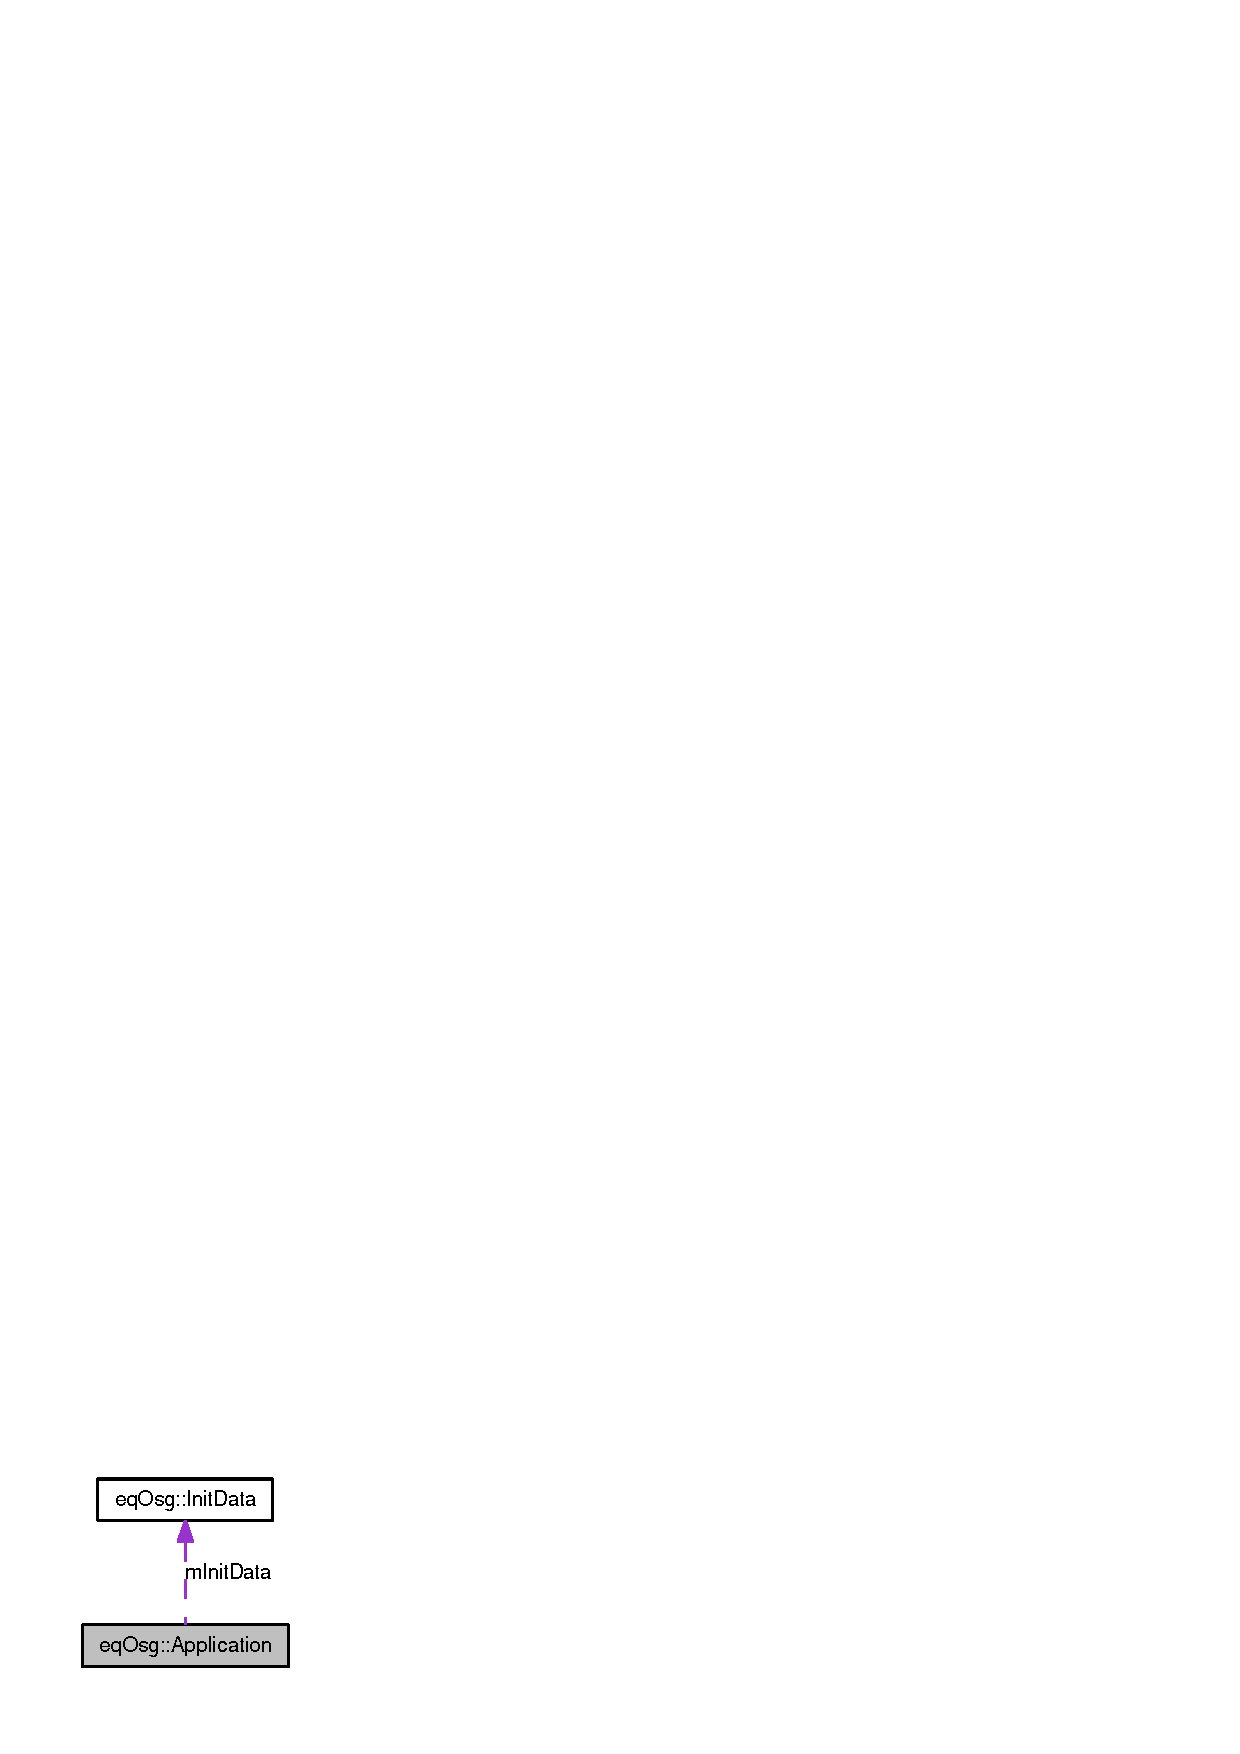
\includegraphics[width=142pt]{a00083}
\end{center}
\end{figure}
\subsection*{Public Member Functions}
\begin{CompactItemize}
\item 
\hyperlink{a00001_004ad4bb523a1a7ffe7a3e53c3eb82e2}{Application} (const \hyperlink{a00011}{InitData} \&initData)
\begin{CompactList}\small\item\em Constructor to pass the init data class. \item\end{CompactList}\item 
\hypertarget{a00001_8cf8941c8db90117d3735bce5ae1fdf4}{
int \hyperlink{a00001_8cf8941c8db90117d3735bce5ae1fdf4}{run} ()}
\label{a00001_8cf8941c8db90117d3735bce5ae1fdf4}

\begin{CompactList}\small\item\em Run this equalizer application. \item\end{CompactList}\end{CompactItemize}
\subsection*{Protected Member Functions}
\begin{CompactItemize}
\item 
\hypertarget{a00001_8b3cb53c57a36c01761b4fe74f9adbb0}{
virtual bool \hyperlink{a00001_8b3cb53c57a36c01761b4fe74f9adbb0}{clientLoop} ()}
\label{a00001_8b3cb53c57a36c01761b4fe74f9adbb0}

\begin{CompactList}\small\item\em The equalizer client loop. \item\end{CompactList}\end{CompactItemize}


\subsection{Detailed Description}
Sets up the whole \hyperlink{a00045}{eqOsg} Equalizer application. 

Contains the Equalizer main loop. 

\subsection{Constructor \& Destructor Documentation}
\hypertarget{a00001_004ad4bb523a1a7ffe7a3e53c3eb82e2}{
\index{eqOsg::Application@{eqOsg::Application}!Application@{Application}}
\index{Application@{Application}!eqOsg::Application@{eqOsg::Application}}
\subsubsection[{Application}]{\setlength{\rightskip}{0pt plus 5cm}Application::Application (const {\bf InitData} \& {\em initData})}}
\label{a00001_004ad4bb523a1a7ffe7a3e53c3eb82e2}


Constructor to pass the init data class. 

\begin{Desc}
\item[Parameters:]
\begin{description}
\item[{\em initData}]The destributet init data object \end{description}
\end{Desc}


The documentation for this class was generated from the following files:\begin{CompactItemize}
\item 
E:/schule/Thesis/Repo/trunk/crf/src/Application.h\item 
E:/schule/Thesis/Repo/trunk/crf/src/Application.cpp\end{CompactItemize}

\hypertarget{a00002}{
\section{eqOsg::Channel Class Reference}
\label{a00002}\index{eqOsg::Channel@{eqOsg::Channel}}
}
The \hyperlink{a00002}{Channel} renders the frames in \hyperlink{a00002_70cfd22742da9b9aa3e3478f356ba220}{frameDraw()}.  


{\tt \#include $<$Channel.h$>$}

Collaboration diagram for eqOsg::Channel:\nopagebreak
\begin{figure}[H]
\begin{center}
\leavevmode
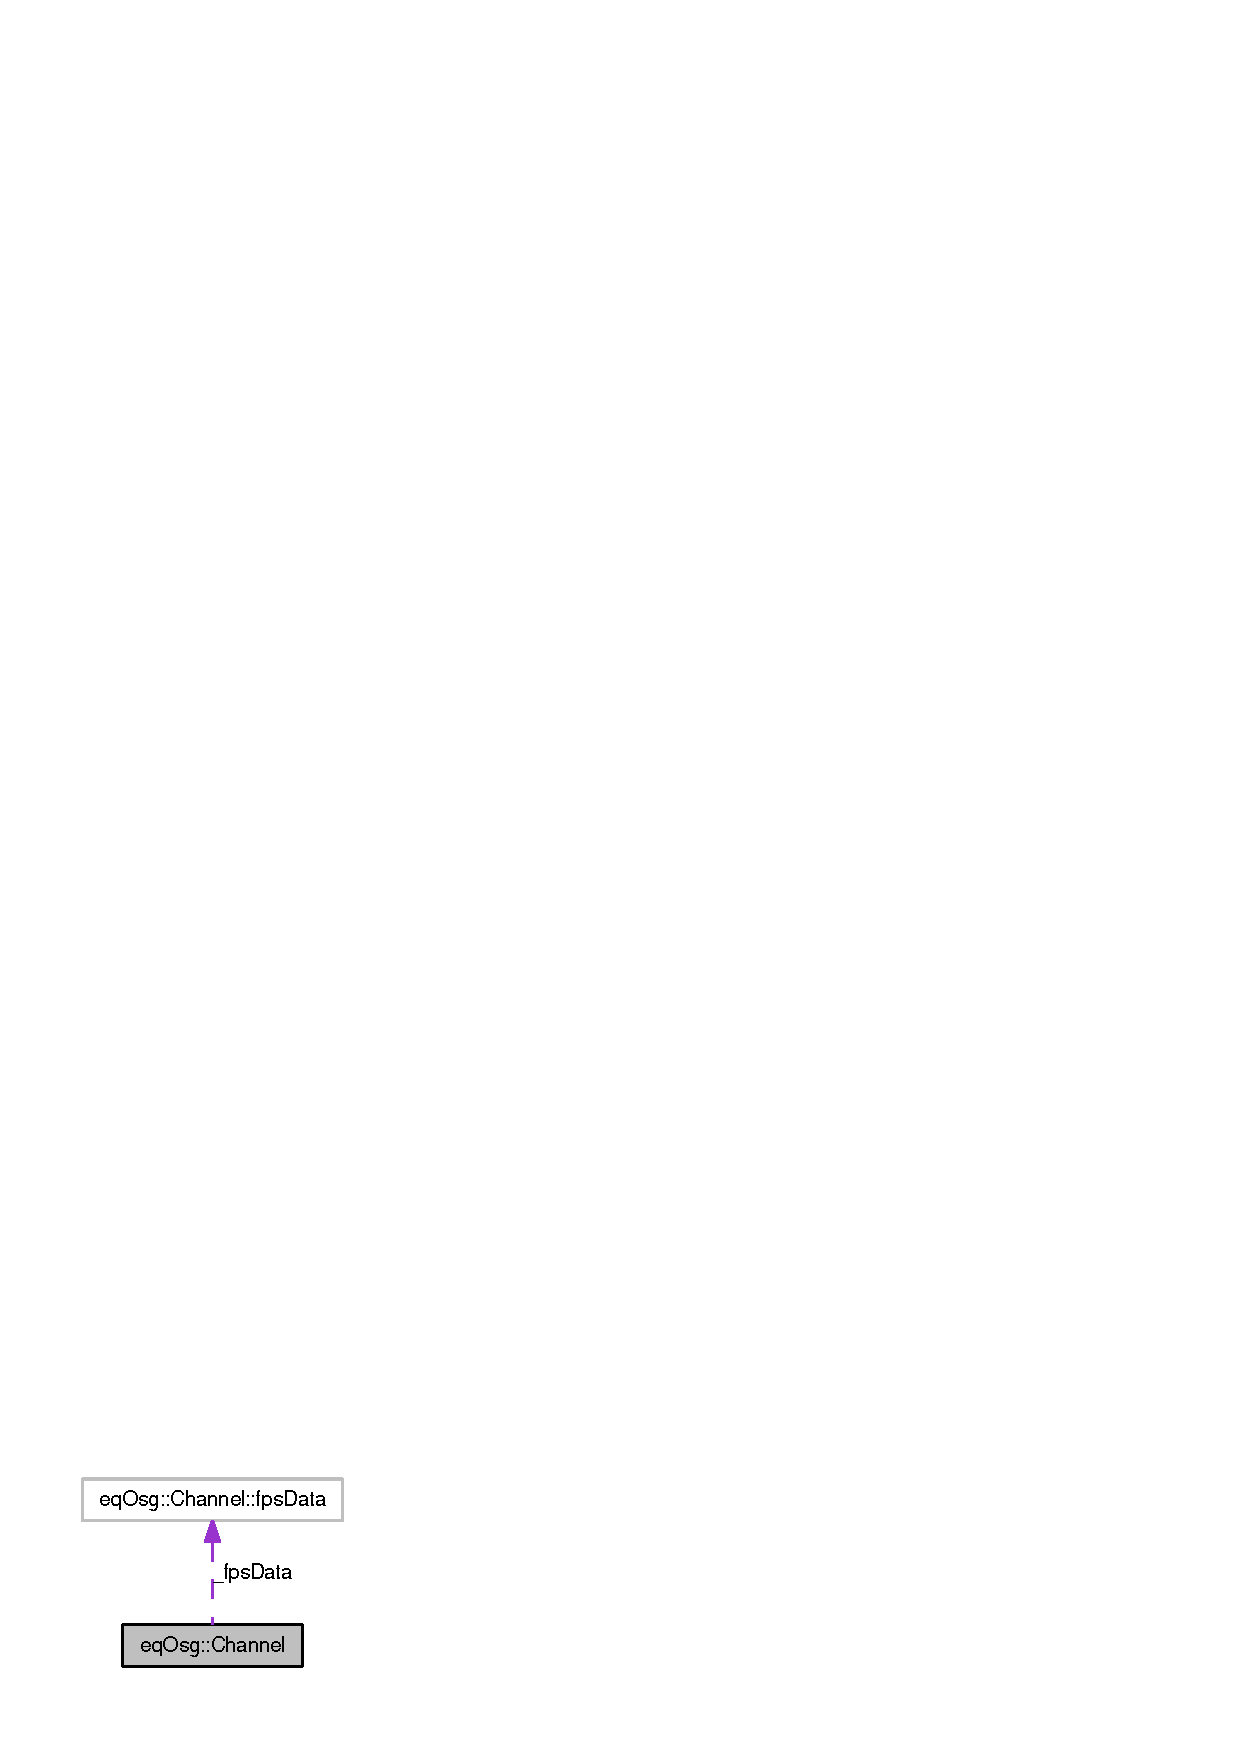
\includegraphics[width=168pt]{a00087}
\end{center}
\end{figure}
\subsection*{Classes}
\begin{CompactItemize}
\item 
struct \textbf{fpsData}
\begin{CompactList}\small\item\em framecounter stuff \item\end{CompactList}\end{CompactItemize}
\subsection*{Public Member Functions}
\begin{CompactItemize}
\item 
\hyperlink{a00002_332b524bf3dd36fb43ff699fb8b64052}{Channel} (eq::Window $\ast$parent)
\begin{CompactList}\small\item\em Creates a channel and sets its parent window. \item\end{CompactList}\end{CompactItemize}
\subsection*{Protected Member Functions}
\begin{CompactItemize}
\item 
virtual void \hyperlink{a00002_70cfd22742da9b9aa3e3478f356ba220}{frameDraw} (const uint32\_\-t frameID)
\begin{CompactList}\small\item\em Renders the scene graph. \item\end{CompactList}\item 
virtual bool \hyperlink{a00002_15ff8d6c9962d86d886dba9485082dde}{configInit} (const uint32\_\-t initID)
\begin{CompactList}\small\item\em \hyperlink{a00003}{Config} initialisation. \item\end{CompactList}\item 
osg::Matrix \hyperlink{a00002_d3a369c393e8065327ef37cef65e25c7}{setPlainViewMatrix} (const \hyperlink{a00014}{Pipe} $\ast$frameData) const 
\begin{CompactList}\small\item\em This function gets the camera position and viewing direction information out of the frame data and sets the view matrix of the camera of the viewer of the pipe based on this information. \item\end{CompactList}\item 
\hypertarget{a00002_2950f8b33948b9f8fea20910b95fc695}{
virtual void \hyperlink{a00002_2950f8b33948b9f8fea20910b95fc695}{drawFPS} ()}
\label{a00002_2950f8b33948b9f8fea20910b95fc695}

\begin{CompactList}\small\item\em Prints the self calculated FPS value. \item\end{CompactList}\item 
\hypertarget{a00002_e0efffd06ae7a755b7f0c80641d5e6d7}{
virtual void \hyperlink{a00002_e0efffd06ae7a755b7f0c80641d5e6d7}{drawInfoText} (std::string txt)}
\label{a00002_e0efffd06ae7a755b7f0c80641d5e6d7}

\begin{CompactList}\small\item\em Prints the channel's info Text. \item\end{CompactList}\end{CompactItemize}


\subsection{Detailed Description}
The \hyperlink{a00002}{Channel} renders the frames in \hyperlink{a00002_70cfd22742da9b9aa3e3478f356ba220}{frameDraw()}. 

This is done by querying the pipe for the viewer and then asking the viewer to render the scene. 

\subsection{Constructor \& Destructor Documentation}
\hypertarget{a00002_332b524bf3dd36fb43ff699fb8b64052}{
\index{eqOsg::Channel@{eqOsg::Channel}!Channel@{Channel}}
\index{Channel@{Channel}!eqOsg::Channel@{eqOsg::Channel}}
\subsubsection[{Channel}]{\setlength{\rightskip}{0pt plus 5cm}Channel::Channel (eq::Window $\ast$ {\em parent})}}
\label{a00002_332b524bf3dd36fb43ff699fb8b64052}


Creates a channel and sets its parent window. 

\begin{Desc}
\item[Parameters:]
\begin{description}
\item[{\em parent}]The equalizer parent window. \end{description}
\end{Desc}


\subsection{Member Function Documentation}
\hypertarget{a00002_15ff8d6c9962d86d886dba9485082dde}{
\index{eqOsg::Channel@{eqOsg::Channel}!configInit@{configInit}}
\index{configInit@{configInit}!eqOsg::Channel@{eqOsg::Channel}}
\subsubsection[{configInit}]{\setlength{\rightskip}{0pt plus 5cm}bool Channel::configInit (const uint32\_\-t {\em initID})\hspace{0.3cm}{\tt  \mbox{[}protected, virtual\mbox{]}}}}
\label{a00002_15ff8d6c9962d86d886dba9485082dde}


\hyperlink{a00003}{Config} initialisation. 

\begin{Desc}
\item[Parameters:]
\begin{description}
\item[{\em initID}]The initID of the config. \end{description}
\end{Desc}
\begin{Desc}
\item[Returns:]True if succeed. \end{Desc}
\hypertarget{a00002_70cfd22742da9b9aa3e3478f356ba220}{
\index{eqOsg::Channel@{eqOsg::Channel}!frameDraw@{frameDraw}}
\index{frameDraw@{frameDraw}!eqOsg::Channel@{eqOsg::Channel}}
\subsubsection[{frameDraw}]{\setlength{\rightskip}{0pt plus 5cm}void Channel::frameDraw (const uint32\_\-t {\em frameID})\hspace{0.3cm}{\tt  \mbox{[}protected, virtual\mbox{]}}}}
\label{a00002_70cfd22742da9b9aa3e3478f356ba220}


Renders the scene graph. 

Draw the frame. Calls \hyperlink{a00002_2950f8b33948b9f8fea20910b95fc695}{drawFPS()}, \hyperlink{a00002_e0efffd06ae7a755b7f0c80641d5e6d7}{drawInfoText()} and eq::Channel::drawStatistics(). \begin{Desc}
\item[Parameters:]
\begin{description}
\item[{\em frameID}]The frame's id to render. \end{description}
\end{Desc}
\hypertarget{a00002_d3a369c393e8065327ef37cef65e25c7}{
\index{eqOsg::Channel@{eqOsg::Channel}!setPlainViewMatrix@{setPlainViewMatrix}}
\index{setPlainViewMatrix@{setPlainViewMatrix}!eqOsg::Channel@{eqOsg::Channel}}
\subsubsection[{setPlainViewMatrix}]{\setlength{\rightskip}{0pt plus 5cm}osg::Matrix Channel::setPlainViewMatrix (const {\bf Pipe} $\ast$ {\em frameData}) const\hspace{0.3cm}{\tt  \mbox{[}protected\mbox{]}}}}
\label{a00002_d3a369c393e8065327ef37cef65e25c7}


This function gets the camera position and viewing direction information out of the frame data and sets the view matrix of the camera of the viewer of the pipe based on this information. 

This view matrix is then also returned. \begin{Desc}
\item[Parameters:]
\begin{description}
\item[{\em frameData}]The pipe which holds the \hyperlink{a00010}{FrameData} Object to get the camera's position. \end{description}
\end{Desc}
\begin{Desc}
\item[Returns:]The newly calculated matrix \end{Desc}


The documentation for this class was generated from the following files:\begin{CompactItemize}
\item 
E:/schule/Thesis/Repo/trunk/crf/src/Channel.h\item 
E:/schule/Thesis/Repo/trunk/crf/src/Channel.cpp\end{CompactItemize}

\hypertarget{a00003}{
\section{eqOsg::Config Class Reference}
\label{a00003}\index{eqOsg::Config@{eqOsg::Config}}
}
This class handles the \hyperlink{a00045}{eqOsg} basic config for Equalizer.  


{\tt \#include $<$Config.h$>$}

Inherited by \hyperlink{a00004}{crf::crfConfig}.

Collaboration diagram for eqOsg::Config:\nopagebreak
\begin{figure}[H]
\begin{center}
\leavevmode
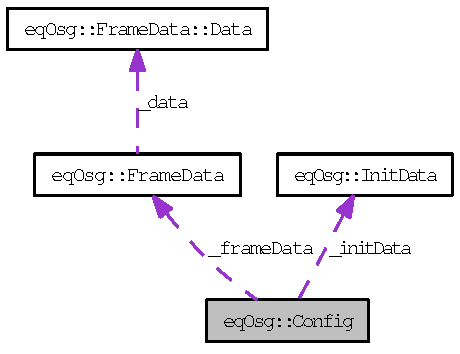
\includegraphics[width=257pt]{a00090}
\end{center}
\end{figure}
\subsection*{Public Member Functions}
\begin{CompactItemize}
\item 
\hyperlink{a00003_64865580c67831fd92e8c5222f0554cc}{Config} (eq::base::RefPtr$<$ eq::Server $>$ parent)
\begin{CompactList}\small\item\em Calls the base constructor and initialises the camera. \item\end{CompactList}\item 
virtual bool \hyperlink{a00003_73ab12bbf273fd4ff7e2dea65ee3e6f8}{init} ()
\begin{CompactList}\small\item\em Initialises our distributet data and calls the eq::Config::init(). \item\end{CompactList}\item 
virtual bool \hyperlink{a00003_e656952f262b9e5c3354583a04068b97}{exit} ()
\begin{CompactList}\small\item\em When exiting the configuration, the distributed data gets deregistered after the base eq::Config::exit() was called. \item\end{CompactList}\item 
virtual uint32\_\-t \hyperlink{a00003_955b3c5ffe177012da10434fbc8da7e0}{startFrame} ()
\begin{CompactList}\small\item\em Starts the new frame for rendering. \item\end{CompactList}\item 
virtual bool \hyperlink{a00003_0ac41bd28010ff7f7638beb051b6c9b9}{handleEvent} (const eq::ConfigEvent $\ast$event)
\begin{CompactList}\small\item\em Reimplemented for camera controls. \item\end{CompactList}\item 
virtual void \hyperlink{a00003_eac7f3b423d994667bac2007c5d78cc1}{setInitData} (const \hyperlink{a00011}{InitData} \&data)
\begin{CompactList}\small\item\em Reimplemented to register the framedata object. \item\end{CompactList}\item 
const \hyperlink{a00011}{InitData} \& \hyperlink{a00003_8a5b1862bf80067322a3a0b1f530f751}{getInitData} () const 
\begin{CompactList}\small\item\em Returns the initData. \item\end{CompactList}\item 
bool \hyperlink{a00003_140db32dd04daba4cb95233e180b0327}{mapData} (const uint32\_\-t initDataID)
\begin{CompactList}\small\item\em Maps our initData. \item\end{CompactList}\end{CompactItemize}
\subsection*{Protected Member Functions}
\begin{CompactItemize}
\item 
virtual void \hyperlink{a00003_b7754b48a74e7927643d3e2e6ca3c8ed}{updateCamera} (float elapsed)
\begin{CompactList}\small\item\em calculates the new properties for the camera \item\end{CompactList}\item 
\hypertarget{a00003_be9b795ee7263d5e8343fbd4c7a00ded}{
virtual void \hyperlink{a00003_be9b795ee7263d5e8343fbd4c7a00ded}{updateFrameData} ()}
\label{a00003_be9b795ee7263d5e8343fbd4c7a00ded}

\begin{CompactList}\small\item\em adds the new properties for framedata \item\end{CompactList}\item 
virtual bool \hyperlink{a00003_b66ac34d32b4e160ec19cb39231395ac}{handleCameraEvents} (const eq::ConfigEvent $\ast$event)
\begin{CompactList}\small\item\em If a keypress happens, this function updates \_\-moveDirection, so that the new camera position can be calculated in \hyperlink{a00003_b7754b48a74e7927643d3e2e6ca3c8ed}{updateCamera()}. \item\end{CompactList}\end{CompactItemize}
\subsection*{Protected Attributes}
\begin{CompactItemize}
\item 
\hypertarget{a00003_26a7379aa8c578f1bd7d404256b70932}{
\hyperlink{a00010}{FrameData} \hyperlink{a00003_26a7379aa8c578f1bd7d404256b70932}{\_\-frameData}}
\label{a00003_26a7379aa8c578f1bd7d404256b70932}

\begin{CompactList}\small\item\em The distributed frame data. \item\end{CompactList}\end{CompactItemize}


\subsection{Detailed Description}
This class handles the \hyperlink{a00045}{eqOsg} basic config for Equalizer. 

The Equalizer related event handling is done here. The \hyperlink{a00045}{eqOsg} basic camera calculations are done here as well. \begin{Desc}
\item[See also:]eq::Config \end{Desc}


\subsection{Constructor \& Destructor Documentation}
\hypertarget{a00003_64865580c67831fd92e8c5222f0554cc}{
\index{eqOsg::Config@{eqOsg::Config}!Config@{Config}}
\index{Config@{Config}!eqOsg::Config@{eqOsg::Config}}
\subsubsection[{Config}]{\setlength{\rightskip}{0pt plus 5cm}Config::Config (eq::base::RefPtr$<$ eq::Server $>$ {\em parent})}}
\label{a00003_64865580c67831fd92e8c5222f0554cc}


Calls the base constructor and initialises the camera. 

\begin{Desc}
\item[See also:]eq::Config::Config \end{Desc}


\subsection{Member Function Documentation}
\hypertarget{a00003_e656952f262b9e5c3354583a04068b97}{
\index{eqOsg::Config@{eqOsg::Config}!exit@{exit}}
\index{exit@{exit}!eqOsg::Config@{eqOsg::Config}}
\subsubsection[{exit}]{\setlength{\rightskip}{0pt plus 5cm}bool Config::exit ()\hspace{0.3cm}{\tt  \mbox{[}virtual\mbox{]}}}}
\label{a00003_e656952f262b9e5c3354583a04068b97}


When exiting the configuration, the distributed data gets deregistered after the base eq::Config::exit() was called. 

\begin{Desc}
\item[Returns:]True if everything worked fine. \end{Desc}
\hypertarget{a00003_8a5b1862bf80067322a3a0b1f530f751}{
\index{eqOsg::Config@{eqOsg::Config}!getInitData@{getInitData}}
\index{getInitData@{getInitData}!eqOsg::Config@{eqOsg::Config}}
\subsubsection[{getInitData}]{\setlength{\rightskip}{0pt plus 5cm}const {\bf InitData} \& Config::getInitData () const}}
\label{a00003_8a5b1862bf80067322a3a0b1f530f751}


Returns the initData. 

\begin{Desc}
\item[Returns:]The initData object. \end{Desc}
\hypertarget{a00003_b66ac34d32b4e160ec19cb39231395ac}{
\index{eqOsg::Config@{eqOsg::Config}!handleCameraEvents@{handleCameraEvents}}
\index{handleCameraEvents@{handleCameraEvents}!eqOsg::Config@{eqOsg::Config}}
\subsubsection[{handleCameraEvents}]{\setlength{\rightskip}{0pt plus 5cm}bool Config::handleCameraEvents (const eq::ConfigEvent $\ast$ {\em event})\hspace{0.3cm}{\tt  \mbox{[}protected, virtual\mbox{]}}}}
\label{a00003_b66ac34d32b4e160ec19cb39231395ac}


If a keypress happens, this function updates \_\-moveDirection, so that the new camera position can be calculated in \hyperlink{a00003_b7754b48a74e7927643d3e2e6ca3c8ed}{updateCamera()}. 

If a mouse move event happens, this function updates \_\-pointerXDiff and \_\-pointerYDiff, so that the new camera viewing direction can be calculated in \hyperlink{a00003_b7754b48a74e7927643d3e2e6ca3c8ed}{updateCamera()}. \begin{Desc}
\item[Parameters:]
\begin{description}
\item[{\em event}]The Equalizer event. \end{description}
\end{Desc}
\begin{Desc}
\item[Returns:]True if the event has been handled. \end{Desc}
\hypertarget{a00003_0ac41bd28010ff7f7638beb051b6c9b9}{
\index{eqOsg::Config@{eqOsg::Config}!handleEvent@{handleEvent}}
\index{handleEvent@{handleEvent}!eqOsg::Config@{eqOsg::Config}}
\subsubsection[{handleEvent}]{\setlength{\rightskip}{0pt plus 5cm}bool Config::handleEvent (const eq::ConfigEvent $\ast$ {\em event})\hspace{0.3cm}{\tt  \mbox{[}virtual\mbox{]}}}}
\label{a00003_0ac41bd28010ff7f7638beb051b6c9b9}


Reimplemented for camera controls. 

Handles the Equalizer events. If camera is enabled handleCameraEvents gets called \begin{Desc}
\item[Parameters:]
\begin{description}
\item[{\em event}]The event passed by Equalizer. \end{description}
\end{Desc}
\begin{Desc}
\item[Returns:]True, if the event has been handled \end{Desc}


toggle the eq cam switch

Update the cameras proberties by handling these events 

Reimplemented in \hyperlink{a00004_63938a0cf75d236b677c4cb147933b3c}{crf::crfConfig}.\hypertarget{a00003_73ab12bbf273fd4ff7e2dea65ee3e6f8}{
\index{eqOsg::Config@{eqOsg::Config}!init@{init}}
\index{init@{init}!eqOsg::Config@{eqOsg::Config}}
\subsubsection[{init}]{\setlength{\rightskip}{0pt plus 5cm}bool Config::init ()\hspace{0.3cm}{\tt  \mbox{[}virtual\mbox{]}}}}
\label{a00003_73ab12bbf273fd4ff7e2dea65ee3e6f8}


Initialises our distributet data and calls the eq::Config::init(). 

\begin{Desc}
\item[Returns:]True if everything succeed. \end{Desc}
\hypertarget{a00003_140db32dd04daba4cb95233e180b0327}{
\index{eqOsg::Config@{eqOsg::Config}!mapData@{mapData}}
\index{mapData@{mapData}!eqOsg::Config@{eqOsg::Config}}
\subsubsection[{mapData}]{\setlength{\rightskip}{0pt plus 5cm}bool Config::mapData (const uint32\_\-t {\em initDataID})}}
\label{a00003_140db32dd04daba4cb95233e180b0327}


Maps our initData. 

\begin{Desc}
\item[Parameters:]
\begin{description}
\item[{\em initDataID}]The initData's ID. \end{description}
\end{Desc}
\begin{Desc}
\item[Returns:]True if everything worked fine. \end{Desc}
\hypertarget{a00003_eac7f3b423d994667bac2007c5d78cc1}{
\index{eqOsg::Config@{eqOsg::Config}!setInitData@{setInitData}}
\index{setInitData@{setInitData}!eqOsg::Config@{eqOsg::Config}}
\subsubsection[{setInitData}]{\setlength{\rightskip}{0pt plus 5cm}void Config::setInitData (const {\bf InitData} \& {\em data})\hspace{0.3cm}{\tt  \mbox{[}virtual\mbox{]}}}}
\label{a00003_eac7f3b423d994667bac2007c5d78cc1}


Reimplemented to register the framedata object. 

\begin{Desc}
\item[Parameters:]
\begin{description}
\item[{\em data}]The init data object. \end{description}
\end{Desc}
\hypertarget{a00003_955b3c5ffe177012da10434fbc8da7e0}{
\index{eqOsg::Config@{eqOsg::Config}!startFrame@{startFrame}}
\index{startFrame@{startFrame}!eqOsg::Config@{eqOsg::Config}}
\subsubsection[{startFrame}]{\setlength{\rightskip}{0pt plus 5cm}uint32\_\-t Config::startFrame ()\hspace{0.3cm}{\tt  \mbox{[}virtual\mbox{]}}}}
\label{a00003_955b3c5ffe177012da10434fbc8da7e0}


Starts the new frame for rendering. 

Camera gets updated with the elapsed time, the frameData gets commited and the base startFrame function gets called. \begin{Desc}
\item[Returns:]Returns the frames ID \end{Desc}
\hypertarget{a00003_b7754b48a74e7927643d3e2e6ca3c8ed}{
\index{eqOsg::Config@{eqOsg::Config}!updateCamera@{updateCamera}}
\index{updateCamera@{updateCamera}!eqOsg::Config@{eqOsg::Config}}
\subsubsection[{updateCamera}]{\setlength{\rightskip}{0pt plus 5cm}void Config::updateCamera (float {\em elapsed})\hspace{0.3cm}{\tt  \mbox{[}protected, virtual\mbox{]}}}}
\label{a00003_b7754b48a74e7927643d3e2e6ca3c8ed}


calculates the new properties for the camera 

\begin{Desc}
\item[Parameters:]
\begin{description}
\item[{\em elapsed}]The elapsed time of th clock to create frame independent movement. \end{description}
\end{Desc}


The documentation for this class was generated from the following files:\begin{CompactItemize}
\item 
E:/schule/Thesis/Repo/trunk/crf/src/Config.h\item 
E:/schule/Thesis/Repo/trunk/crf/src/Config.cpp\end{CompactItemize}

\hypertarget{a00004}{
\section{crf::crfConfig Class Reference}
\label{a00004}\index{crf::crfConfig@{crf::crfConfig}}
}
This class extends the basic \hyperlink{a00045}{eqOsg} config class with support vor event forwarding to the pipe's viewer.  


{\tt \#include $<$crfConfig.h$>$}

Inherits \hyperlink{a00003}{eqOsg::Config}.

Collaboration diagram for crf::crfConfig:\nopagebreak
\begin{figure}[H]
\begin{center}
\leavevmode
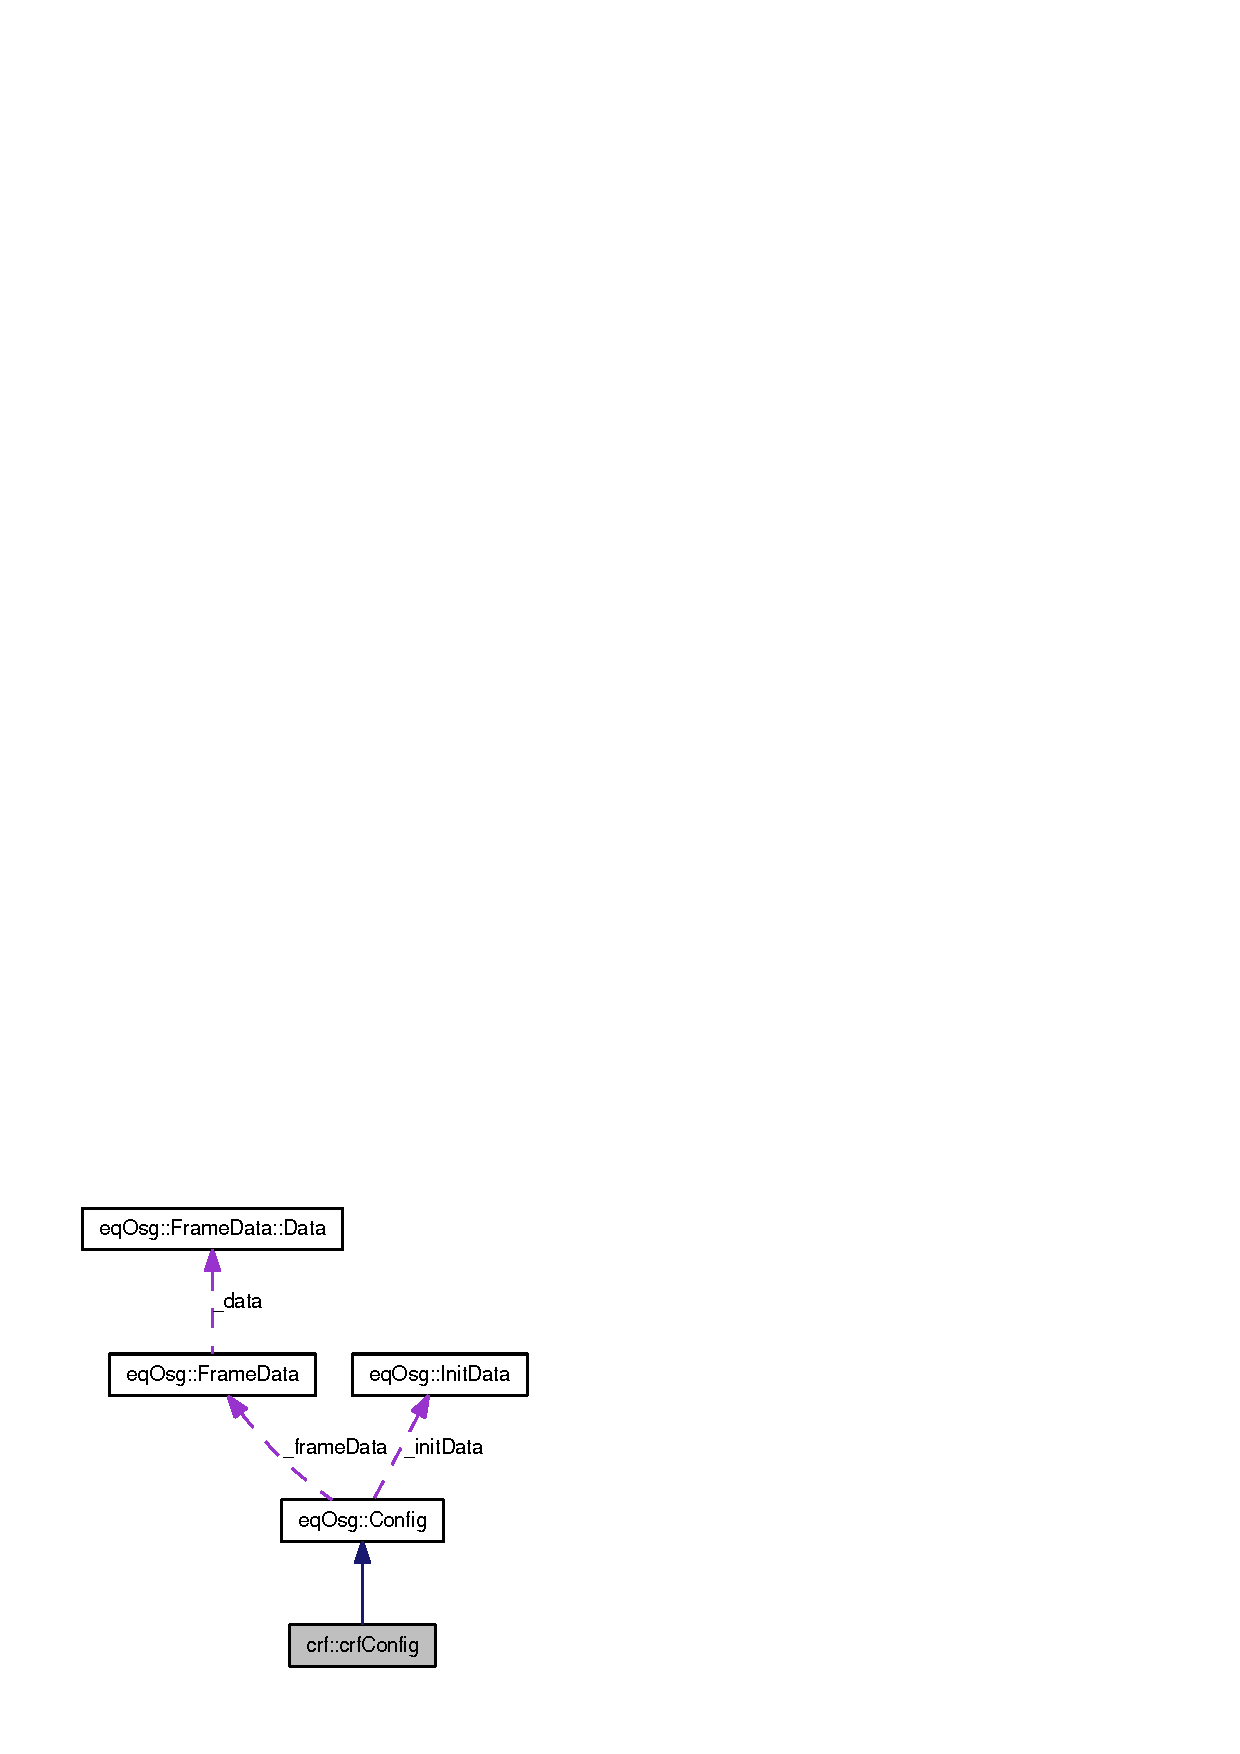
\includegraphics[width=257pt]{a00070}
\end{center}
\end{figure}
\subsection*{Public Member Functions}
\begin{CompactItemize}
\item 
\hyperlink{a00004_3ddcfcc9f305f6e8502078f922d7280f}{crfConfig} (eq::ServerPtr parent)
\item 
virtual bool \hyperlink{a00004_63938a0cf75d236b677c4cb147933b3c}{handleEvent} (const eq::ConfigEvent $\ast$event)
\begin{CompactList}\small\item\em Passes the desired events to the FrameData's event queue and calls the eqOsg::Config::handleEvents function. \item\end{CompactList}\item 
virtual uint32\_\-t \hyperlink{a00004_ebe9cfdff7f345f6d1f706be246520f7}{finishFrame} ()
\begin{CompactList}\small\item\em Clears the eventlist in FrameData and calls the base eq::Config::frameFinish(). \item\end{CompactList}\end{CompactItemize}


\subsection{Detailed Description}
This class extends the basic \hyperlink{a00045}{eqOsg} config class with support vor event forwarding to the pipe's viewer. 

\begin{Desc}
\item[See also:]\hyperlink{a00003}{eqOsg::Config} \end{Desc}


\subsection{Constructor \& Destructor Documentation}
\hypertarget{a00004_3ddcfcc9f305f6e8502078f922d7280f}{
\index{crf::crfConfig@{crf::crfConfig}!crfConfig@{crfConfig}}
\index{crfConfig@{crfConfig}!crf::crfConfig@{crf::crfConfig}}
\subsubsection[{crfConfig}]{\setlength{\rightskip}{0pt plus 5cm}crf::crfConfig::crfConfig (eq::ServerPtr {\em parent})\hspace{0.3cm}{\tt  \mbox{[}inline\mbox{]}}}}
\label{a00004_3ddcfcc9f305f6e8502078f922d7280f}


\begin{Desc}
\item[See also:]\hyperlink{a00003}{eqOsg::Config} \end{Desc}


\subsection{Member Function Documentation}
\hypertarget{a00004_ebe9cfdff7f345f6d1f706be246520f7}{
\index{crf::crfConfig@{crf::crfConfig}!finishFrame@{finishFrame}}
\index{finishFrame@{finishFrame}!crf::crfConfig@{crf::crfConfig}}
\subsubsection[{finishFrame}]{\setlength{\rightskip}{0pt plus 5cm}uint32\_\-t crf::crfConfig::finishFrame ()\hspace{0.3cm}{\tt  \mbox{[}virtual\mbox{]}}}}
\label{a00004_ebe9cfdff7f345f6d1f706be246520f7}


Clears the eventlist in FrameData and calls the base eq::Config::frameFinish(). 

\begin{Desc}
\item[Returns:]The finished frame's number. \end{Desc}
\begin{Desc}
\item[See also:]eq::Config::finishFrame \end{Desc}
\hypertarget{a00004_63938a0cf75d236b677c4cb147933b3c}{
\index{crf::crfConfig@{crf::crfConfig}!handleEvent@{handleEvent}}
\index{handleEvent@{handleEvent}!crf::crfConfig@{crf::crfConfig}}
\subsubsection[{handleEvent}]{\setlength{\rightskip}{0pt plus 5cm}bool crf::crfConfig::handleEvent (const eq::ConfigEvent $\ast$ {\em event})\hspace{0.3cm}{\tt  \mbox{[}virtual\mbox{]}}}}
\label{a00004_63938a0cf75d236b677c4cb147933b3c}


Passes the desired events to the FrameData's event queue and calls the eqOsg::Config::handleEvents function. 

\begin{Desc}
\item[Parameters:]
\begin{description}
\item[{\em event}]The to handle event. \end{description}
\end{Desc}
\begin{Desc}
\item[Returns:]True if the an event has been handled. \end{Desc}
\begin{Desc}
\item[See also:]eqOsg::Config::hanleEvent() \end{Desc}


Pass the mouse and keyboard events to framedata

Mouse events 

Reimplemented from \hyperlink{a00003_0ac41bd28010ff7f7638beb051b6c9b9}{eqOsg::Config}.

The documentation for this class was generated from the following files:\begin{CompactItemize}
\item 
E:/schule/Thesis/Repo/trunk/crf/src/crfConfig.h\item 
E:/schule/Thesis/Repo/trunk/crf/src/crfConfig.cpp\end{CompactItemize}

\hypertarget{a00005}{
\section{crf::crfNodeFactory Class Reference}
\label{a00005}\index{crf::crfNodeFactory@{crf::crfNodeFactory}}
}
This class generates the \hyperlink{a00043}{crf} Equalizer objects.  


{\tt \#include $<$crfNodeFactory.h$>$}

Inherits \hyperlink{a00013}{eqOsg::NodeFactory}.

Collaboration diagram for crf::crfNodeFactory:\nopagebreak
\begin{figure}[H]
\begin{center}
\leavevmode
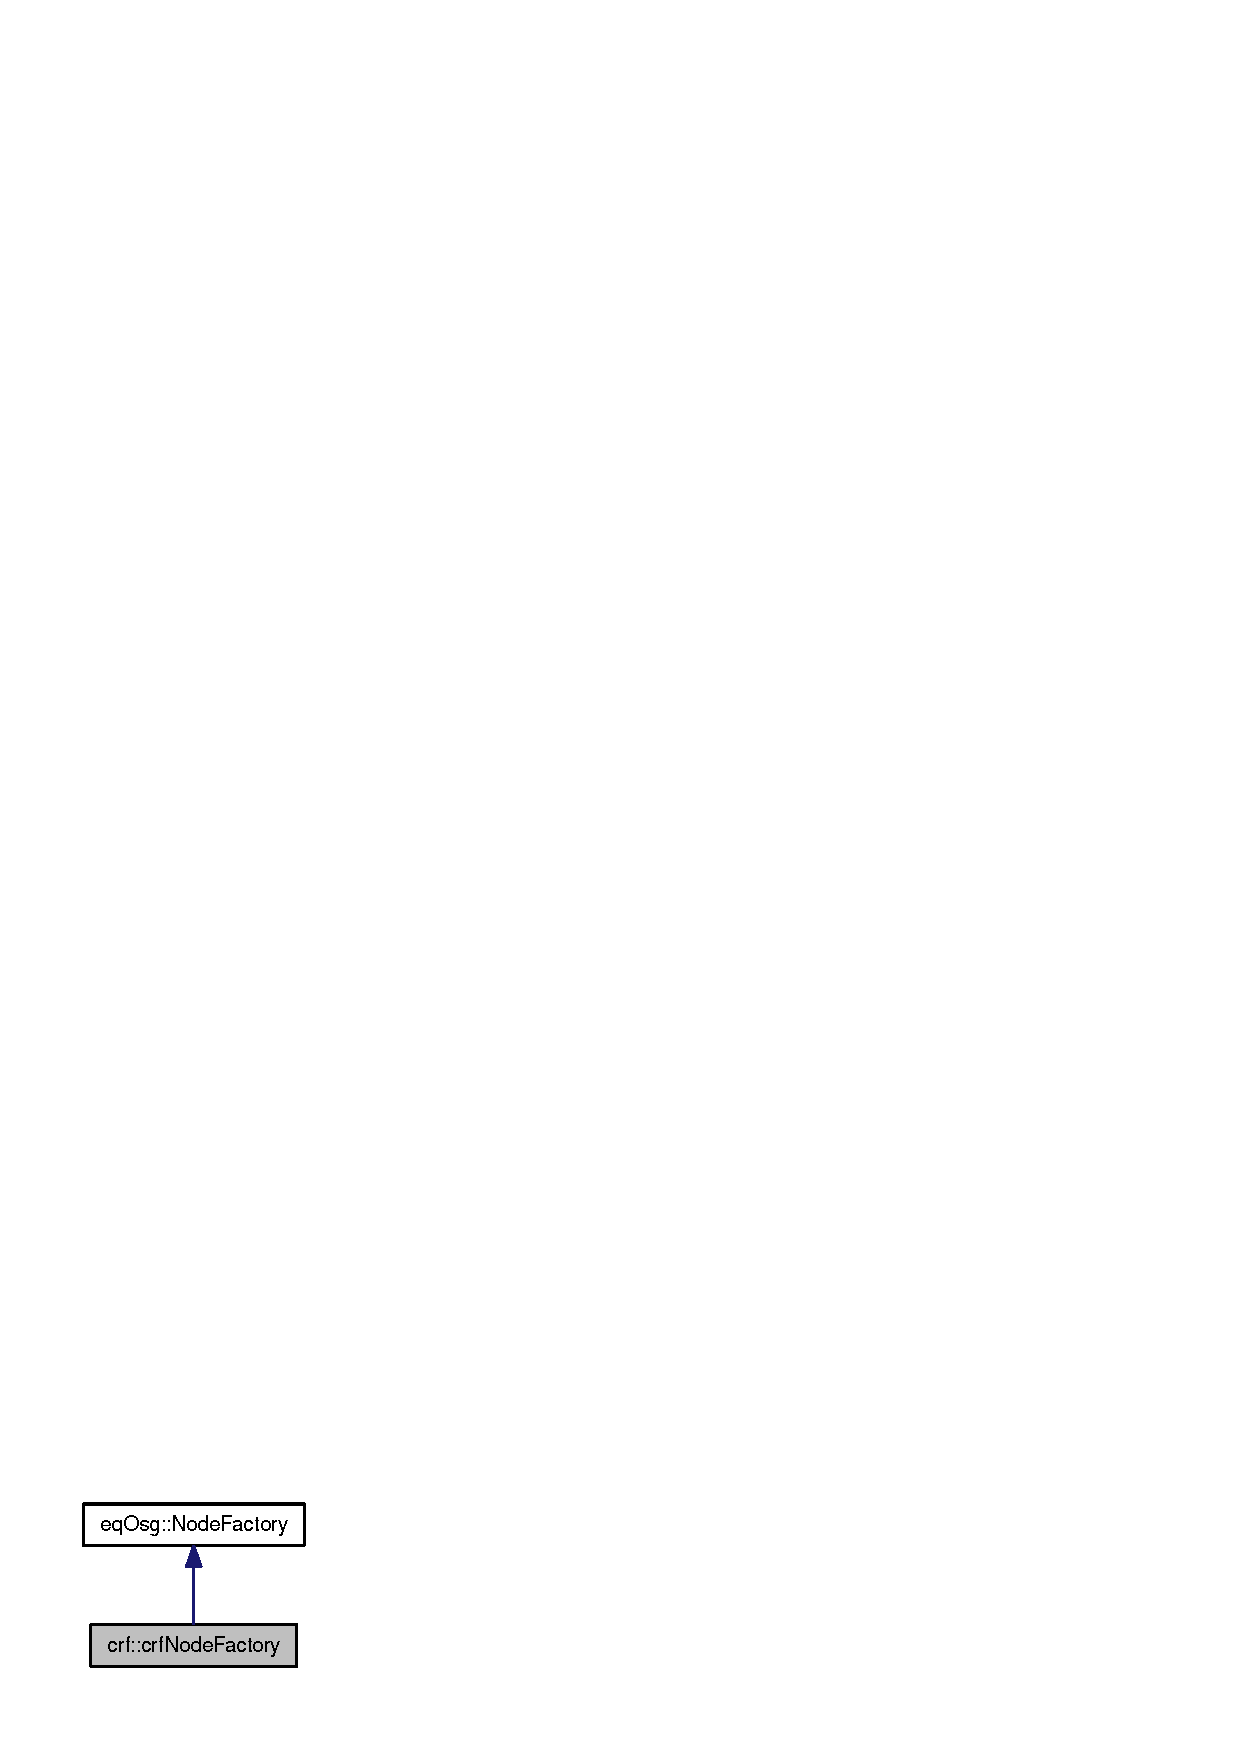
\includegraphics[width=150pt]{a00073}
\end{center}
\end{figure}
\subsection*{Public Member Functions}
\begin{CompactItemize}
\item 
\hypertarget{a00005_1361d01b702cda3adc2dc149fd4b9e58}{
\hyperlink{a00005_1361d01b702cda3adc2dc149fd4b9e58}{crfNodeFactory} ()}
\label{a00005_1361d01b702cda3adc2dc149fd4b9e58}

\begin{CompactList}\small\item\em Sets the sceneNode pointer to zero. \item\end{CompactList}\item 
virtual eq::Pipe $\ast$ \hyperlink{a00005_5f35c307f323b385869226c6083df93d}{createPipe} (eq::Node $\ast$parent)
\begin{CompactList}\small\item\em Creates the \hyperlink{a00006}{crfPipe} objects. \item\end{CompactList}\item 
virtual eq::Config $\ast$ \hyperlink{a00005_0b7b562ae3d0ccc5a98017195926057f}{createConfig} (eq::ServerPtr parent)
\begin{CompactList}\small\item\em Initialises the \hyperlink{a00004}{crfConfig}. \item\end{CompactList}\item 
void \hyperlink{a00005_52740ca913279f9cbdfc4a10f55b691d}{setSceneNode} (osg::ref\_\-ptr$<$ osg::Node $>$ node)
\begin{CompactList}\small\item\em Sets the pipes root node. \item\end{CompactList}\end{CompactItemize}


\subsection{Detailed Description}
This class generates the \hyperlink{a00043}{crf} Equalizer objects. 

\begin{Desc}
\item[See also:]\hyperlink{a00013}{eqOsg::NodeFactory} \end{Desc}


\subsection{Member Function Documentation}
\hypertarget{a00005_0b7b562ae3d0ccc5a98017195926057f}{
\index{crf::crfNodeFactory@{crf::crfNodeFactory}!createConfig@{createConfig}}
\index{createConfig@{createConfig}!crf::crfNodeFactory@{crf::crfNodeFactory}}
\subsubsection[{createConfig}]{\setlength{\rightskip}{0pt plus 5cm}virtual eq::Config$\ast$ crf::crfNodeFactory::createConfig (eq::ServerPtr {\em parent})\hspace{0.3cm}{\tt  \mbox{[}inline, virtual\mbox{]}}}}
\label{a00005_0b7b562ae3d0ccc5a98017195926057f}


Initialises the \hyperlink{a00004}{crfConfig}. 

\begin{Desc}
\item[See also:]eqOsg::Nodefactory::createConfig \end{Desc}


Reimplemented from \hyperlink{a00013_0e80614084de6b23a4a2677fc8af7f93}{eqOsg::NodeFactory}.\hypertarget{a00005_5f35c307f323b385869226c6083df93d}{
\index{crf::crfNodeFactory@{crf::crfNodeFactory}!createPipe@{createPipe}}
\index{createPipe@{createPipe}!crf::crfNodeFactory@{crf::crfNodeFactory}}
\subsubsection[{createPipe}]{\setlength{\rightskip}{0pt plus 5cm}virtual eq::Pipe$\ast$ crf::crfNodeFactory::createPipe (eq::Node $\ast$ {\em parent})\hspace{0.3cm}{\tt  \mbox{[}inline, virtual\mbox{]}}}}
\label{a00005_5f35c307f323b385869226c6083df93d}


Creates the \hyperlink{a00006}{crfPipe} objects. 

If a osg::Node is set, the node will be passed to the new pipe. \begin{Desc}
\item[See also:]\hyperlink{a00013_10e06f5d0d32f146994274682d39e666}{eqOsg::NodeFactory::createPipe} \end{Desc}


Reimplemented from \hyperlink{a00013_10e06f5d0d32f146994274682d39e666}{eqOsg::NodeFactory}.\hypertarget{a00005_52740ca913279f9cbdfc4a10f55b691d}{
\index{crf::crfNodeFactory@{crf::crfNodeFactory}!setSceneNode@{setSceneNode}}
\index{setSceneNode@{setSceneNode}!crf::crfNodeFactory@{crf::crfNodeFactory}}
\subsubsection[{setSceneNode}]{\setlength{\rightskip}{0pt plus 5cm}void crf::crfNodeFactory::setSceneNode (osg::ref\_\-ptr$<$ osg::Node $>$ {\em node})\hspace{0.3cm}{\tt  \mbox{[}inline\mbox{]}}}}
\label{a00005_52740ca913279f9cbdfc4a10f55b691d}


Sets the pipes root node. 

If this node is set, this node will be passed to the pipe. \begin{Desc}
\item[Parameters:]
\begin{description}
\item[{\em node}]The to set osg scene node \end{description}
\end{Desc}


The documentation for this class was generated from the following file:\begin{CompactItemize}
\item 
E:/schule/Thesis/Repo/trunk/crf/src/crfNodeFactory.h\end{CompactItemize}

\hypertarget{a00006}{
\section{crf::crfPipe Class Reference}
\label{a00006}\index{crf::crfPipe@{crf::crfPipe}}
}
The \hyperlink{a00043}{crf} pipe inherits from the basic \hyperlink{a00045}{eqOsg} pipe, to add more features like event-adapting, scenegraph updates etc.  


{\tt \#include $<$crfPipe.h$>$}

Inherits \hyperlink{a00014}{eqOsg::Pipe}.

Collaboration diagram for crf::crfPipe:\nopagebreak
\begin{figure}[H]
\begin{center}
\leavevmode
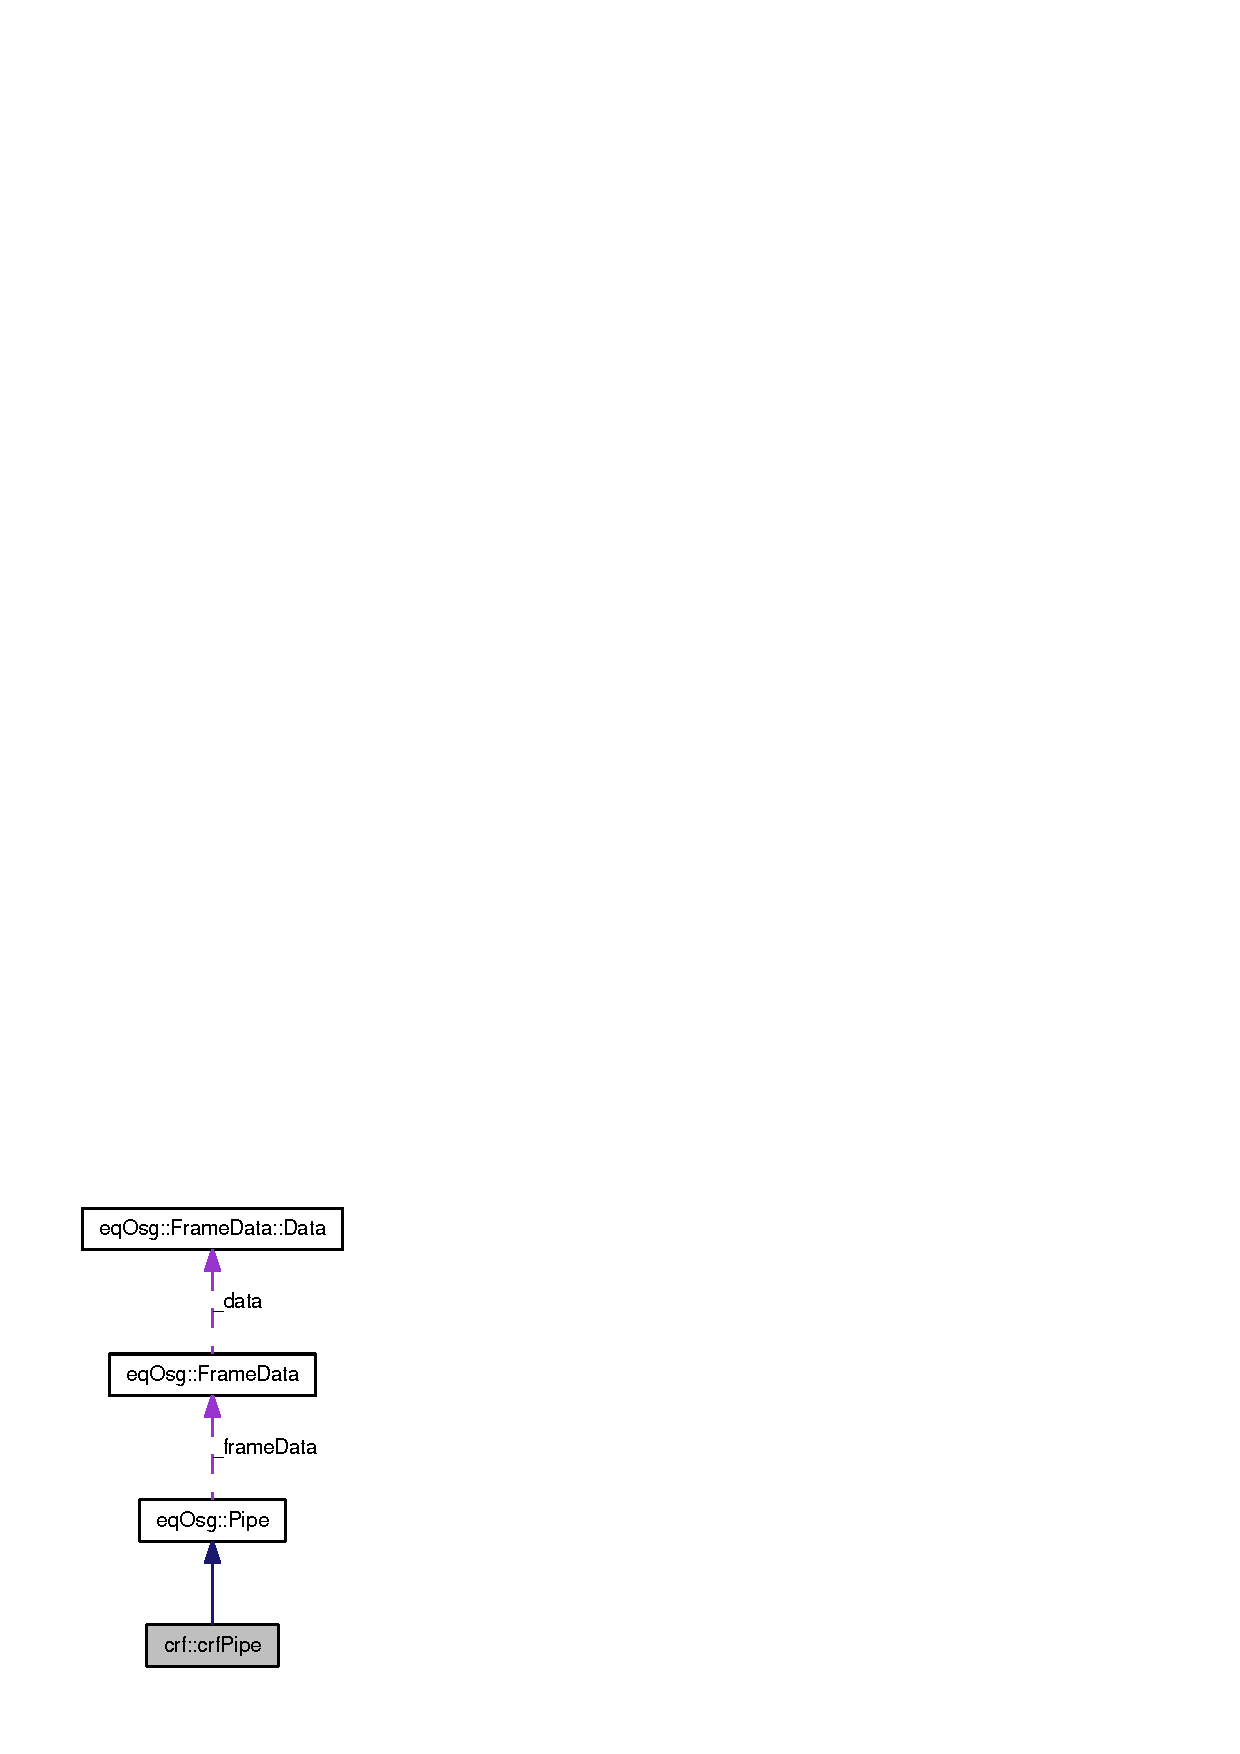
\includegraphics[width=168pt]{a00076}
\end{center}
\end{figure}
\subsection*{Public Member Functions}
\begin{CompactItemize}
\item 
\hyperlink{a00006_0b43238e38fb190f8a5e9a6148950ea0}{crfPipe} (eq::Node $\ast$parent)
\begin{CompactList}\small\item\em Creates a pipe with the empty viewer. \item\end{CompactList}\item 
\hyperlink{a00006_f5c46c7219b170979654b9e0defda4a7}{crfPipe} (eq::Node $\ast$parent, osg::ref\_\-ptr$<$ \hyperlink{a00009}{eqOsg::EqViewer} $>$ viewer)
\begin{CompactList}\small\item\em Creates a pipe with a given viewer. \item\end{CompactList}\item 
\hyperlink{a00006_d1215b24804515699867f0e718eb6985}{crfPipe} (eq::Node $\ast$parent, osg::ref\_\-ptr$<$ osg::Node $>$ sceneNode)
\begin{CompactList}\small\item\em Creates a pipe with a given osg scene node. \item\end{CompactList}\end{CompactItemize}
\subsection*{Protected Member Functions}
\begin{CompactItemize}
\item 
virtual void \hyperlink{a00006_2e551fe08841da2b7a1def541656d48c}{frameStart} (const uint32\_\-t frameID, const uint32\_\-t frameNumber)
\begin{CompactList}\small\item\em Starts the frame and calls converEqEventsToOsg(). \item\end{CompactList}\item 
virtual bool \hyperlink{a00006_fcf11863d5370a815bd7e1216cc0f2e6}{configInit} (const uint32\_\-t initID)
\begin{CompactList}\small\item\em Called when pipe gets initalised. \item\end{CompactList}\item 
virtual void \hyperlink{a00006_16ff3017a9a333b3c7dd21b2032567c4}{convertEqEventsToOsg} ()
\begin{CompactList}\small\item\em Take the eq-events out of the \_\-eventQueue in FrameData and pass it to the eqViewer. \item\end{CompactList}\item 
virtual void \hyperlink{a00006_44e473d6aa40bdb24ae85f1dfd1f973d}{createSceneGraph} ()
\begin{CompactList}\small\item\em Override this function to create the scene graph. \item\end{CompactList}\item 
virtual void \hyperlink{a00006_5288fedad120ffd32f3290b4c91065b7}{updateSceneGraph} ()
\begin{CompactList}\small\item\em Updates your scenegraph at the end of every frame. \item\end{CompactList}\item 
virtual void \hyperlink{a00006_44ac49a7ba2b74a56b00177009d09c93}{setUpViewer} ()
\begin{CompactList}\small\item\em This functions sets up the viewer. \item\end{CompactList}\item 
virtual void \hyperlink{a00006_61564c072f120d8898e57cb268118f9a}{convertKeyPressEvents} (eq::Event event)
\begin{CompactList}\small\item\em Convert the key press events. \item\end{CompactList}\item 
virtual void \hyperlink{a00006_9e4c676e2d880a7149d61c13f2e34f73}{convertKeyReleaseEvents} (eq::Event event)
\begin{CompactList}\small\item\em Convert the key release events. \item\end{CompactList}\item 
virtual void \hyperlink{a00006_bdce51a794891a4b0caa3f33ba6e7ab4}{convertMouseEvents} (eq::Event event)
\begin{CompactList}\small\item\em Converts the key press events. \item\end{CompactList}\item 
virtual bool \hyperlink{a00006_3f48f5f5a8a455342b111f26ca1402db}{configExit} ()
\begin{CompactList}\small\item\em Unref the viewer when closing. \item\end{CompactList}\end{CompactItemize}


\subsection{Detailed Description}
The \hyperlink{a00043}{crf} pipe inherits from the basic \hyperlink{a00045}{eqOsg} pipe, to add more features like event-adapting, scenegraph updates etc. 

Override this class' functions to create your own dynmaic and event depended scene graph. If you do so, don't forget to create your own \hyperlink{a00005}{crfNodeFactory} and pass it to \hyperlink{a00007}{crfStarter}, to force the CRF to use your objects. 

\subsection{Constructor \& Destructor Documentation}
\hypertarget{a00006_0b43238e38fb190f8a5e9a6148950ea0}{
\index{crf::crfPipe@{crf::crfPipe}!crfPipe@{crfPipe}}
\index{crfPipe@{crfPipe}!crf::crfPipe@{crf::crfPipe}}
\subsubsection[{crfPipe}]{\setlength{\rightskip}{0pt plus 5cm}crf::crfPipe::crfPipe (eq::Node $\ast$ {\em parent})\hspace{0.3cm}{\tt  \mbox{[}inline\mbox{]}}}}
\label{a00006_0b43238e38fb190f8a5e9a6148950ea0}


Creates a pipe with the empty viewer. 

Sets \_\-sceneGraphCreated to false! \begin{Desc}
\item[Parameters:]
\begin{description}
\item[{\em parent}]The pipe's Parent (a node). \end{description}
\end{Desc}
\begin{Desc}
\item[See also:]\hyperlink{a00014}{eqOsg::Pipe} \end{Desc}
\hypertarget{a00006_f5c46c7219b170979654b9e0defda4a7}{
\index{crf::crfPipe@{crf::crfPipe}!crfPipe@{crfPipe}}
\index{crfPipe@{crfPipe}!crf::crfPipe@{crf::crfPipe}}
\subsubsection[{crfPipe}]{\setlength{\rightskip}{0pt plus 5cm}crfPipe::crfPipe (eq::Node $\ast$ {\em parent}, \/  osg::ref\_\-ptr$<$ {\bf eqOsg::EqViewer} $>$ {\em viewer})}}
\label{a00006_f5c46c7219b170979654b9e0defda4a7}


Creates a pipe with a given viewer. 

\begin{Desc}
\item[See also:]\hyperlink{a00014}{eqOsg::Pipe} \end{Desc}
\begin{Desc}
\item[Parameters:]
\begin{description}
\item[{\em parent}]The pipe's parent. \item[{\em viewer}]The Pointer to a complete independent \hyperlink{a00009}{eqOsg::EqViewer}. \end{description}
\end{Desc}
\hypertarget{a00006_d1215b24804515699867f0e718eb6985}{
\index{crf::crfPipe@{crf::crfPipe}!crfPipe@{crfPipe}}
\index{crfPipe@{crfPipe}!crf::crfPipe@{crf::crfPipe}}
\subsubsection[{crfPipe}]{\setlength{\rightskip}{0pt plus 5cm}crfPipe::crfPipe (eq::Node $\ast$ {\em parent}, \/  osg::ref\_\-ptr$<$ osg::Node $>$ {\em sceneNode})}}
\label{a00006_d1215b24804515699867f0e718eb6985}


Creates a pipe with a given osg scene node. 

\begin{Desc}
\item[See also:]\hyperlink{a00014}{eqOsg::Pipe} \end{Desc}
\begin{Desc}
\item[Parameters:]
\begin{description}
\item[{\em parent}]The pipe's parent. \item[{\em sceneNode}]The scene node to display. This osg node is gonna be insereted as sceneData to the EqViewer. \end{description}
\end{Desc}


\subsection{Member Function Documentation}
\hypertarget{a00006_3f48f5f5a8a455342b111f26ca1402db}{
\index{crf::crfPipe@{crf::crfPipe}!configExit@{configExit}}
\index{configExit@{configExit}!crf::crfPipe@{crf::crfPipe}}
\subsubsection[{configExit}]{\setlength{\rightskip}{0pt plus 5cm}bool crfPipe::configExit ()\hspace{0.3cm}{\tt  \mbox{[}protected, virtual\mbox{]}}}}
\label{a00006_3f48f5f5a8a455342b111f26ca1402db}


Unref the viewer when closing. 

\begin{Desc}
\item[Returns:]True if everything worked fine. \end{Desc}
\begin{Desc}
\item[See also:]eqOsg::configExit \end{Desc}


Reimplemented from \hyperlink{a00014_2cb47387a7be185b1dc6d097dc4da38e}{eqOsg::Pipe}.\hypertarget{a00006_fcf11863d5370a815bd7e1216cc0f2e6}{
\index{crf::crfPipe@{crf::crfPipe}!configInit@{configInit}}
\index{configInit@{configInit}!crf::crfPipe@{crf::crfPipe}}
\subsubsection[{configInit}]{\setlength{\rightskip}{0pt plus 5cm}bool crfPipe::configInit (const uint32\_\-t {\em initID})\hspace{0.3cm}{\tt  \mbox{[}protected, virtual\mbox{]}}}}
\label{a00006_fcf11863d5370a815bd7e1216cc0f2e6}


Called when pipe gets initalised. 

CreateSceneGraph() is called here if \_\-sceneGraphCreated is still set to false. \begin{Desc}
\item[Returns:]True if everything worked fine. \end{Desc}
\begin{Desc}
\item[See also:]eqOsg::configInit \end{Desc}


Reimplemented from \hyperlink{a00014_d23bd6f7bb0f59f94fc0e279dbbb9d9a}{eqOsg::Pipe}.\hypertarget{a00006_16ff3017a9a333b3c7dd21b2032567c4}{
\index{crf::crfPipe@{crf::crfPipe}!convertEqEventsToOsg@{convertEqEventsToOsg}}
\index{convertEqEventsToOsg@{convertEqEventsToOsg}!crf::crfPipe@{crf::crfPipe}}
\subsubsection[{convertEqEventsToOsg}]{\setlength{\rightskip}{0pt plus 5cm}void crfPipe::convertEqEventsToOsg ()\hspace{0.3cm}{\tt  \mbox{[}protected, virtual\mbox{]}}}}
\label{a00006_16ff3017a9a333b3c7dd21b2032567c4}


Take the eq-events out of the \_\-eventQueue in FrameData and pass it to the eqViewer. 

Basic implementation, converts only basic keys yet.

This function can be OS depended, because eq does not report the same ascii codes for every windowing system! Actually all basic keys and some special keys are forewarded to the osg viewer. In Windows, the pushed ascii codes represent upper case letters. \hypertarget{a00006_61564c072f120d8898e57cb268118f9a}{
\index{crf::crfPipe@{crf::crfPipe}!convertKeyPressEvents@{convertKeyPressEvents}}
\index{convertKeyPressEvents@{convertKeyPressEvents}!crf::crfPipe@{crf::crfPipe}}
\subsubsection[{convertKeyPressEvents}]{\setlength{\rightskip}{0pt plus 5cm}void crfPipe::convertKeyPressEvents (eq::Event {\em event})\hspace{0.3cm}{\tt  \mbox{[}protected, virtual\mbox{]}}}}
\label{a00006_61564c072f120d8898e57cb268118f9a}


Convert the key press events. 

\begin{Desc}
\item[Parameters:]
\begin{description}
\item[{\em event}]The eq event to convert \end{description}
\end{Desc}
\hypertarget{a00006_9e4c676e2d880a7149d61c13f2e34f73}{
\index{crf::crfPipe@{crf::crfPipe}!convertKeyReleaseEvents@{convertKeyReleaseEvents}}
\index{convertKeyReleaseEvents@{convertKeyReleaseEvents}!crf::crfPipe@{crf::crfPipe}}
\subsubsection[{convertKeyReleaseEvents}]{\setlength{\rightskip}{0pt plus 5cm}void crfPipe::convertKeyReleaseEvents (eq::Event {\em event})\hspace{0.3cm}{\tt  \mbox{[}protected, virtual\mbox{]}}}}
\label{a00006_9e4c676e2d880a7149d61c13f2e34f73}


Convert the key release events. 

convert the key release events

\begin{Desc}
\item[Parameters:]
\begin{description}
\item[{\em event}]The eq event to convert \end{description}
\end{Desc}
\hypertarget{a00006_bdce51a794891a4b0caa3f33ba6e7ab4}{
\index{crf::crfPipe@{crf::crfPipe}!convertMouseEvents@{convertMouseEvents}}
\index{convertMouseEvents@{convertMouseEvents}!crf::crfPipe@{crf::crfPipe}}
\subsubsection[{convertMouseEvents}]{\setlength{\rightskip}{0pt plus 5cm}void crfPipe::convertMouseEvents (eq::Event {\em event})\hspace{0.3cm}{\tt  \mbox{[}protected, virtual\mbox{]}}}}
\label{a00006_bdce51a794891a4b0caa3f33ba6e7ab4}


Converts the key press events. 

convert the mouse events

\begin{Desc}
\item[Parameters:]
\begin{description}
\item[{\em event}]The eq event to convert \end{description}
\end{Desc}
\hypertarget{a00006_44e473d6aa40bdb24ae85f1dfd1f973d}{
\index{crf::crfPipe@{crf::crfPipe}!createSceneGraph@{createSceneGraph}}
\index{createSceneGraph@{createSceneGraph}!crf::crfPipe@{crf::crfPipe}}
\subsubsection[{createSceneGraph}]{\setlength{\rightskip}{0pt plus 5cm}void crfPipe::createSceneGraph ()\hspace{0.3cm}{\tt  \mbox{[}protected, virtual\mbox{]}}}}
\label{a00006_44e473d6aa40bdb24ae85f1dfd1f973d}


Override this function to create the scene graph. 

Pass the root node of the scene graph to the \_\-viewer member, add OSG eventhandlers if desired etc... \hypertarget{a00006_2e551fe08841da2b7a1def541656d48c}{
\index{crf::crfPipe@{crf::crfPipe}!frameStart@{frameStart}}
\index{frameStart@{frameStart}!crf::crfPipe@{crf::crfPipe}}
\subsubsection[{frameStart}]{\setlength{\rightskip}{0pt plus 5cm}void crfPipe::frameStart (const uint32\_\-t {\em frameID}, \/  const uint32\_\-t {\em frameNumber})\hspace{0.3cm}{\tt  \mbox{[}protected, virtual\mbox{]}}}}
\label{a00006_2e551fe08841da2b7a1def541656d48c}


Starts the frame and calls converEqEventsToOsg(). 

\begin{Desc}
\item[See also:]eqOsg::Pipe::framestart \end{Desc}


Reimplemented from \hyperlink{a00014_6be431b1b9fe04da31596ea8b870dfde}{eqOsg::Pipe}.\hypertarget{a00006_44ac49a7ba2b74a56b00177009d09c93}{
\index{crf::crfPipe@{crf::crfPipe}!setUpViewer@{setUpViewer}}
\index{setUpViewer@{setUpViewer}!crf::crfPipe@{crf::crfPipe}}
\subsubsection[{setUpViewer}]{\setlength{\rightskip}{0pt plus 5cm}void crfPipe::setUpViewer ()\hspace{0.3cm}{\tt  \mbox{[}protected, virtual\mbox{]}}}}
\label{a00006_44ac49a7ba2b74a56b00177009d09c93}


This functions sets up the viewer. 

Currently an OSG statshandler is added and listen to the F2 keystroke. Override this function to specify your viewer. \hypertarget{a00006_5288fedad120ffd32f3290b4c91065b7}{
\index{crf::crfPipe@{crf::crfPipe}!updateSceneGraph@{updateSceneGraph}}
\index{updateSceneGraph@{updateSceneGraph}!crf::crfPipe@{crf::crfPipe}}
\subsubsection[{updateSceneGraph}]{\setlength{\rightskip}{0pt plus 5cm}virtual void crf::crfPipe::updateSceneGraph ()\hspace{0.3cm}{\tt  \mbox{[}inline, protected, virtual\mbox{]}}}}
\label{a00006_5288fedad120ffd32f3290b4c91065b7}


Updates your scenegraph at the end of every frame. 

Override this function to create your own frame/time related animations. Basic Implementation: empty! 

The documentation for this class was generated from the following files:\begin{CompactItemize}
\item 
E:/schule/Thesis/Repo/trunk/crf/src/crfPipe.h\item 
E:/schule/Thesis/Repo/trunk/crf/src/crfPipe.cpp\end{CompactItemize}

\hypertarget{a00007}{
\section{crf::crfStarter Class Reference}
\label{a00007}\index{crf::crfStarter@{crf::crfStarter}}
}
This class provides easly handable \hyperlink{a00007_bff219a07f93750e4e6db09fd026de7f}{run()} methods to start an equalizer application with OSG scene data.  


{\tt \#include $<$crfStarter.h$>$}

Collaboration diagram for crf::crfStarter:\nopagebreak
\begin{figure}[H]
\begin{center}
\leavevmode
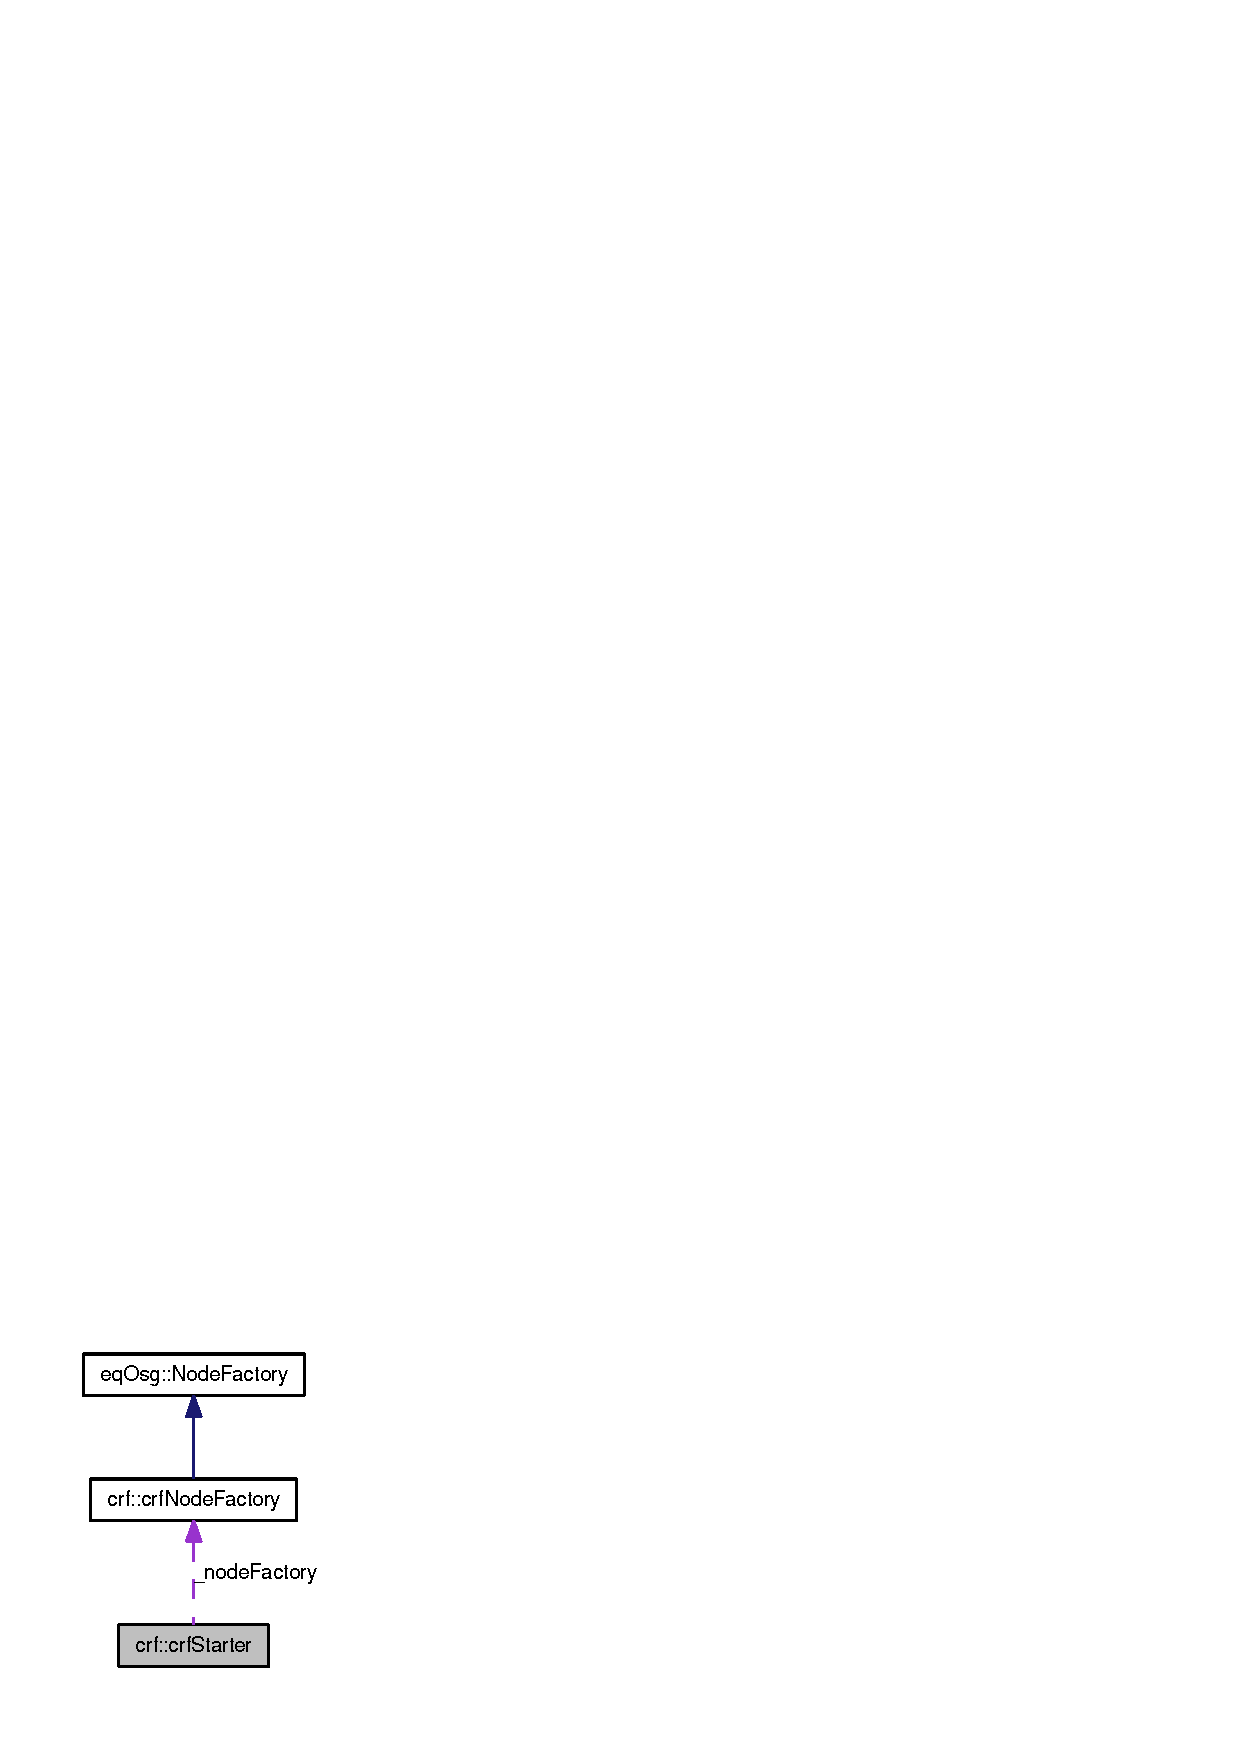
\includegraphics[width=156pt]{a00079}
\end{center}
\end{figure}
\subsection*{Public Member Functions}
\begin{CompactItemize}
\item 
\hypertarget{a00007_e1d24d865b4c98f43163acafc3a48fce}{
\hyperlink{a00007_e1d24d865b4c98f43163acafc3a48fce}{crfStarter} ()}
\label{a00007_e1d24d865b4c98f43163acafc3a48fce}

\begin{CompactList}\small\item\em Default constructor. Sets the viewer- and nodefactorypointer to zero. \item\end{CompactList}\item 
virtual int \hyperlink{a00007_bff219a07f93750e4e6db09fd026de7f}{run} (int argc, char $\ast$$\ast$argv)
\begin{CompactList}\small\item\em Initialize with arguments. \item\end{CompactList}\item 
virtual int \hyperlink{a00007_20c31de1c50c6504a4aaa617d606715b}{run} (int argc, char $\ast$$\ast$argv, osg::ref\_\-ptr$<$ osg::Node $>$ node)
\begin{CompactList}\small\item\em Initialises with arguments and the osg-node which should be displayed with equalizer. \item\end{CompactList}\item 
void \hyperlink{a00007_317832b54784e7c2c21f5d6bda17cda3}{setNodeFactory} (\hyperlink{a00005}{crfNodeFactory} $\ast$fac)
\begin{CompactList}\small\item\em Sets the custom node factory to provide the overriden \hyperlink{a00043}{crf} classes. \item\end{CompactList}\item 
std::string \hyperlink{a00007_b74ff2cc944f29fb91262ab5a9fa084a}{parseCommandLineForString} (int argc, char $\ast$$\ast$argv, std::string prefix)
\begin{CompactList}\small\item\em returns a string minus the passed prefix, if the prefix could be found \item\end{CompactList}\item 
\hyperlink{a00005}{crf::crfNodeFactory} $\ast$ \hyperlink{a00007_6b14742d2d820eba786626ab044c7cbd}{getNodeFactory} ()
\begin{CompactList}\small\item\em Gets the custom node factory. \item\end{CompactList}\end{CompactItemize}


\subsection{Detailed Description}
This class provides easly handable \hyperlink{a00007_bff219a07f93750e4e6db09fd026de7f}{run()} methods to start an equalizer application with OSG scene data. 

Actually these modes are supported: \begin{itemize}
\item Pass an osg::node as 3rd argument. This node will be the scene graph's root node \item Override \hyperlink{a00006}{crfPipe} and other \hyperlink{a00043}{crf} classes to create your more specific scene. Create a \hyperlink{a00005}{crf::crfNodeFactory} which generates the overriden classes and pass it with \hyperlink{a00007_317832b54784e7c2c21f5d6bda17cda3}{crfStarter::setNodeFactory()} to this starter class. \item Do nothing: The \char`\"{}HelloWorld\char`\"{} scene will be rendered.\end{itemize}


\subsection{Member Function Documentation}
\hypertarget{a00007_6b14742d2d820eba786626ab044c7cbd}{
\index{crf::crfStarter@{crf::crfStarter}!getNodeFactory@{getNodeFactory}}
\index{getNodeFactory@{getNodeFactory}!crf::crfStarter@{crf::crfStarter}}
\subsubsection[{getNodeFactory}]{\setlength{\rightskip}{0pt plus 5cm}{\bf crf::crfNodeFactory}$\ast$ crf::crfStarter::getNodeFactory ()\hspace{0.3cm}{\tt  \mbox{[}inline\mbox{]}}}}
\label{a00007_6b14742d2d820eba786626ab044c7cbd}


Gets the custom node factory. 

\begin{Desc}
\item[Returns:]The starter's viewer factory. \end{Desc}
\hypertarget{a00007_b74ff2cc944f29fb91262ab5a9fa084a}{
\index{crf::crfStarter@{crf::crfStarter}!parseCommandLineForString@{parseCommandLineForString}}
\index{parseCommandLineForString@{parseCommandLineForString}!crf::crfStarter@{crf::crfStarter}}
\subsubsection[{parseCommandLineForString}]{\setlength{\rightskip}{0pt plus 5cm}std::string crf::crfStarter::parseCommandLineForString (int {\em argc}, \/  char $\ast$$\ast$ {\em argv}, \/  std::string {\em prefix})}}
\label{a00007_b74ff2cc944f29fb91262ab5a9fa084a}


returns a string minus the passed prefix, if the prefix could be found 

\begin{Desc}
\item[Parameters:]
\begin{description}
\item[{\em argc}]argument counter \item[{\em argv}]command line arguments \item[{\em prefix}]the specified prefix \end{description}
\end{Desc}
\begin{Desc}
\item[Returns:]the to found string withou prefix \end{Desc}
\hypertarget{a00007_20c31de1c50c6504a4aaa617d606715b}{
\index{crf::crfStarter@{crf::crfStarter}!run@{run}}
\index{run@{run}!crf::crfStarter@{crf::crfStarter}}
\subsubsection[{run}]{\setlength{\rightskip}{0pt plus 5cm}virtual int crf::crfStarter::run (int {\em argc}, \/  char $\ast$$\ast$ {\em argv}, \/  osg::ref\_\-ptr$<$ osg::Node $>$ {\em node})\hspace{0.3cm}{\tt  \mbox{[}virtual\mbox{]}}}}
\label{a00007_20c31de1c50c6504a4aaa617d606715b}


Initialises with arguments and the osg-node which should be displayed with equalizer. 

\begin{Desc}
\item[Parameters:]
\begin{description}
\item[{\em argc}]CmdLine Argument Counter \item[{\em argv}]CmdLine Arguments \item[{\em node}]OSG Node \end{description}
\end{Desc}
\begin{Desc}
\item[Returns:]The cpp default main return value. \end{Desc}
\hypertarget{a00007_bff219a07f93750e4e6db09fd026de7f}{
\index{crf::crfStarter@{crf::crfStarter}!run@{run}}
\index{run@{run}!crf::crfStarter@{crf::crfStarter}}
\subsubsection[{run}]{\setlength{\rightskip}{0pt plus 5cm}int crf::crfStarter::run (int {\em argc}, \/  char $\ast$$\ast$ {\em argv})\hspace{0.3cm}{\tt  \mbox{[}virtual\mbox{]}}}}
\label{a00007_bff219a07f93750e4e6db09fd026de7f}


Initialize with arguments. 

\begin{Desc}
\item[Parameters:]
\begin{description}
\item[{\em argc}]CmdLine Argument Counter. \item[{\em argv}]CmdLine Arguments. \end{description}
\end{Desc}
\begin{Desc}
\item[Returns:]The cpp default main return value. \end{Desc}
\hypertarget{a00007_317832b54784e7c2c21f5d6bda17cda3}{
\index{crf::crfStarter@{crf::crfStarter}!setNodeFactory@{setNodeFactory}}
\index{setNodeFactory@{setNodeFactory}!crf::crfStarter@{crf::crfStarter}}
\subsubsection[{setNodeFactory}]{\setlength{\rightskip}{0pt plus 5cm}void crf::crfStarter::setNodeFactory ({\bf crfNodeFactory} $\ast$ {\em fac})\hspace{0.3cm}{\tt  \mbox{[}inline\mbox{]}}}}
\label{a00007_317832b54784e7c2c21f5d6bda17cda3}


Sets the custom node factory to provide the overriden \hyperlink{a00043}{crf} classes. 

\begin{Desc}
\item[Parameters:]
\begin{description}
\item[{\em fac}]The custom node factory. \end{description}
\end{Desc}


The documentation for this class was generated from the following files:\begin{CompactItemize}
\item 
E:/schule/Thesis/Repo/trunk/crf/src/crfStarter.h\item 
E:/schule/Thesis/Repo/trunk/crf/src/crfStarter.cpp\end{CompactItemize}

\hypertarget{a00008}{
\section{eqOsg::FrameData::Data Struct Reference}
\label{a00008}\index{eqOsg::FrameData::Data@{eqOsg::FrameData::Data}}
}
The FrameData's struct to hold members.  


{\tt \#include $<$FrameData.h$>$}

\subsection*{Public Attributes}
\begin{CompactItemize}
\item 
\hypertarget{a00008_a3cfc1223feb27c15704fc3147e97918}{
bool \hyperlink{a00008_a3cfc1223feb27c15704fc3147e97918}{controlEqCam}}
\label{a00008_a3cfc1223feb27c15704fc3147e97918}

\begin{CompactList}\small\item\em eq-camera switch \item\end{CompactList}\item 
\hypertarget{a00008_3d7e162b15c8002297eae09a51d20cb8}{
vmml::Vector3f \hyperlink{a00008_3d7e162b15c8002297eae09a51d20cb8}{cameraPosition}}
\label{a00008_3d7e162b15c8002297eae09a51d20cb8}

\begin{CompactList}\small\item\em The position of the camrra, in world coordinates. \item\end{CompactList}\item 
\hypertarget{a00008_5ddb1c00dd8d5537474e33e234d7b96e}{
vmml::Vector3f \hyperlink{a00008_5ddb1c00dd8d5537474e33e234d7b96e}{cameraLookAtPoint}}
\label{a00008_5ddb1c00dd8d5537474e33e234d7b96e}

\begin{CompactList}\small\item\em The point the camera is looking at, in world coordinates. \item\end{CompactList}\item 
\hypertarget{a00008_720f59f063b8a1ab581918361987ffd4}{
vmml::Vector3f \hyperlink{a00008_720f59f063b8a1ab581918361987ffd4}{cameraUpVector}}
\label{a00008_720f59f063b8a1ab581918361987ffd4}

\begin{CompactList}\small\item\em The up vector of the camera. \item\end{CompactList}\item 
\hypertarget{a00008_53f26b3187a95b3f28be5eaaf7595a1d}{
bool \hyperlink{a00008_53f26b3187a95b3f28be5eaaf7595a1d}{osgTrackBallSwitch}}
\label{a00008_53f26b3187a95b3f28be5eaaf7595a1d}

\begin{CompactList}\small\item\em Enable osg Trackball Manipulator. \item\end{CompactList}\item 
\hypertarget{a00008_bf1897dca052068e3240c5779f5d8944}{
bool \hyperlink{a00008_bf1897dca052068e3240c5779f5d8944}{equalizerStatsSwitch}}
\label{a00008_bf1897dca052068e3240c5779f5d8944}

\begin{CompactList}\small\item\em Enable eq stats. \item\end{CompactList}\item 
\hypertarget{a00008_2d2657de7d24d1921cd9818308ac3106}{
bool \hyperlink{a00008_2d2657de7d24d1921cd9818308ac3106}{crfOverlaySwitch}}
\label{a00008_2d2657de7d24d1921cd9818308ac3106}

\begin{CompactList}\small\item\em Enable crfOverlay. \item\end{CompactList}\item 
\hypertarget{a00008_50fb31217b91cb805acf163645674bcf}{
bool \hyperlink{a00008_50fb31217b91cb805acf163645674bcf}{crfFPSSwitch}}
\label{a00008_50fb31217b91cb805acf163645674bcf}

\begin{CompactList}\small\item\em show \hyperlink{a00043}{crf} FPS \item\end{CompactList}\end{CompactItemize}


\subsection{Detailed Description}
The FrameData's struct to hold members. 

The documentation for this struct was generated from the following file:\begin{CompactItemize}
\item 
E:/schule/Thesis/Repo/trunk/crf/src/FrameData.h\end{CompactItemize}

\hypertarget{a00009}{
\section{eqOsg::EqViewer Class Reference}
\label{a00009}\index{eqOsg::EqViewer@{eqOsg::EqViewer}}
}
A Viewer which can be used with Equalizer.  


{\tt \#include $<$EqViewer.h$>$}

\subsection*{Public Member Functions}
\begin{CompactItemize}
\item 
\hypertarget{a00009_bd6695b9ab0b08062c3d6377ae8ac275}{
\hyperlink{a00009_bd6695b9ab0b08062c3d6377ae8ac275}{EqViewer} ()}
\label{a00009_bd6695b9ab0b08062c3d6377ae8ac275}

\begin{CompactList}\small\item\em Default constructor. Sets the threading model to \char`\"{}Single\char`\"{} because embedded window viewers need this. \item\end{CompactList}\item 
void \hyperlink{a00009_c998d9f70b12556a17396dfdabb2c185}{setViewport} (eq::Channel $\ast$channel)
\begin{CompactList}\small\item\em Sets the viewport of the Camara of the scene so that it matches the viewport of the given Equalizer channel. \item\end{CompactList}\end{CompactItemize}


\subsection{Detailed Description}
A Viewer which can be used with Equalizer. 

A normal Viewer from OSG would try to create its own windows, which we don't want to, since they are set up by Equalizer for us.

The \hyperlink{a00009}{EqViewer} solves this by setting the correct context and viewport.

Call \hyperlink{a00009_c998d9f70b12556a17396dfdabb2c185}{setViewport()} in your frameDraw() method. 

\subsection{Member Function Documentation}
\hypertarget{a00009_c998d9f70b12556a17396dfdabb2c185}{
\index{eqOsg::EqViewer@{eqOsg::EqViewer}!setViewport@{setViewport}}
\index{setViewport@{setViewport}!eqOsg::EqViewer@{eqOsg::EqViewer}}
\subsubsection[{setViewport}]{\setlength{\rightskip}{0pt plus 5cm}void EqViewer::setViewport (eq::Channel $\ast$ {\em channel})}}
\label{a00009_c998d9f70b12556a17396dfdabb2c185}


Sets the viewport of the Camara of the scene so that it matches the viewport of the given Equalizer channel. 

\begin{Desc}
\item[Parameters:]
\begin{description}
\item[{\em channel}]The channel with the Equalizer set viewport. \end{description}
\end{Desc}


The documentation for this class was generated from the following files:\begin{CompactItemize}
\item 
E:/schule/Thesis/Repo/trunk/crf/src/EqViewer.h\item 
E:/schule/Thesis/Repo/trunk/crf/src/EqViewer.cpp\end{CompactItemize}

\hypertarget{a00010}{
\section{eqOsg::FrameData Class Reference}
\label{a00010}\index{eqOsg::FrameData@{eqOsg::FrameData}}
}
\hyperlink{a00010}{FrameData} holds all data which is updated each frame.  


{\tt \#include $<$FrameData.h$>$}

Collaboration diagram for eqOsg::FrameData:\nopagebreak
\begin{figure}[H]
\begin{center}
\leavevmode
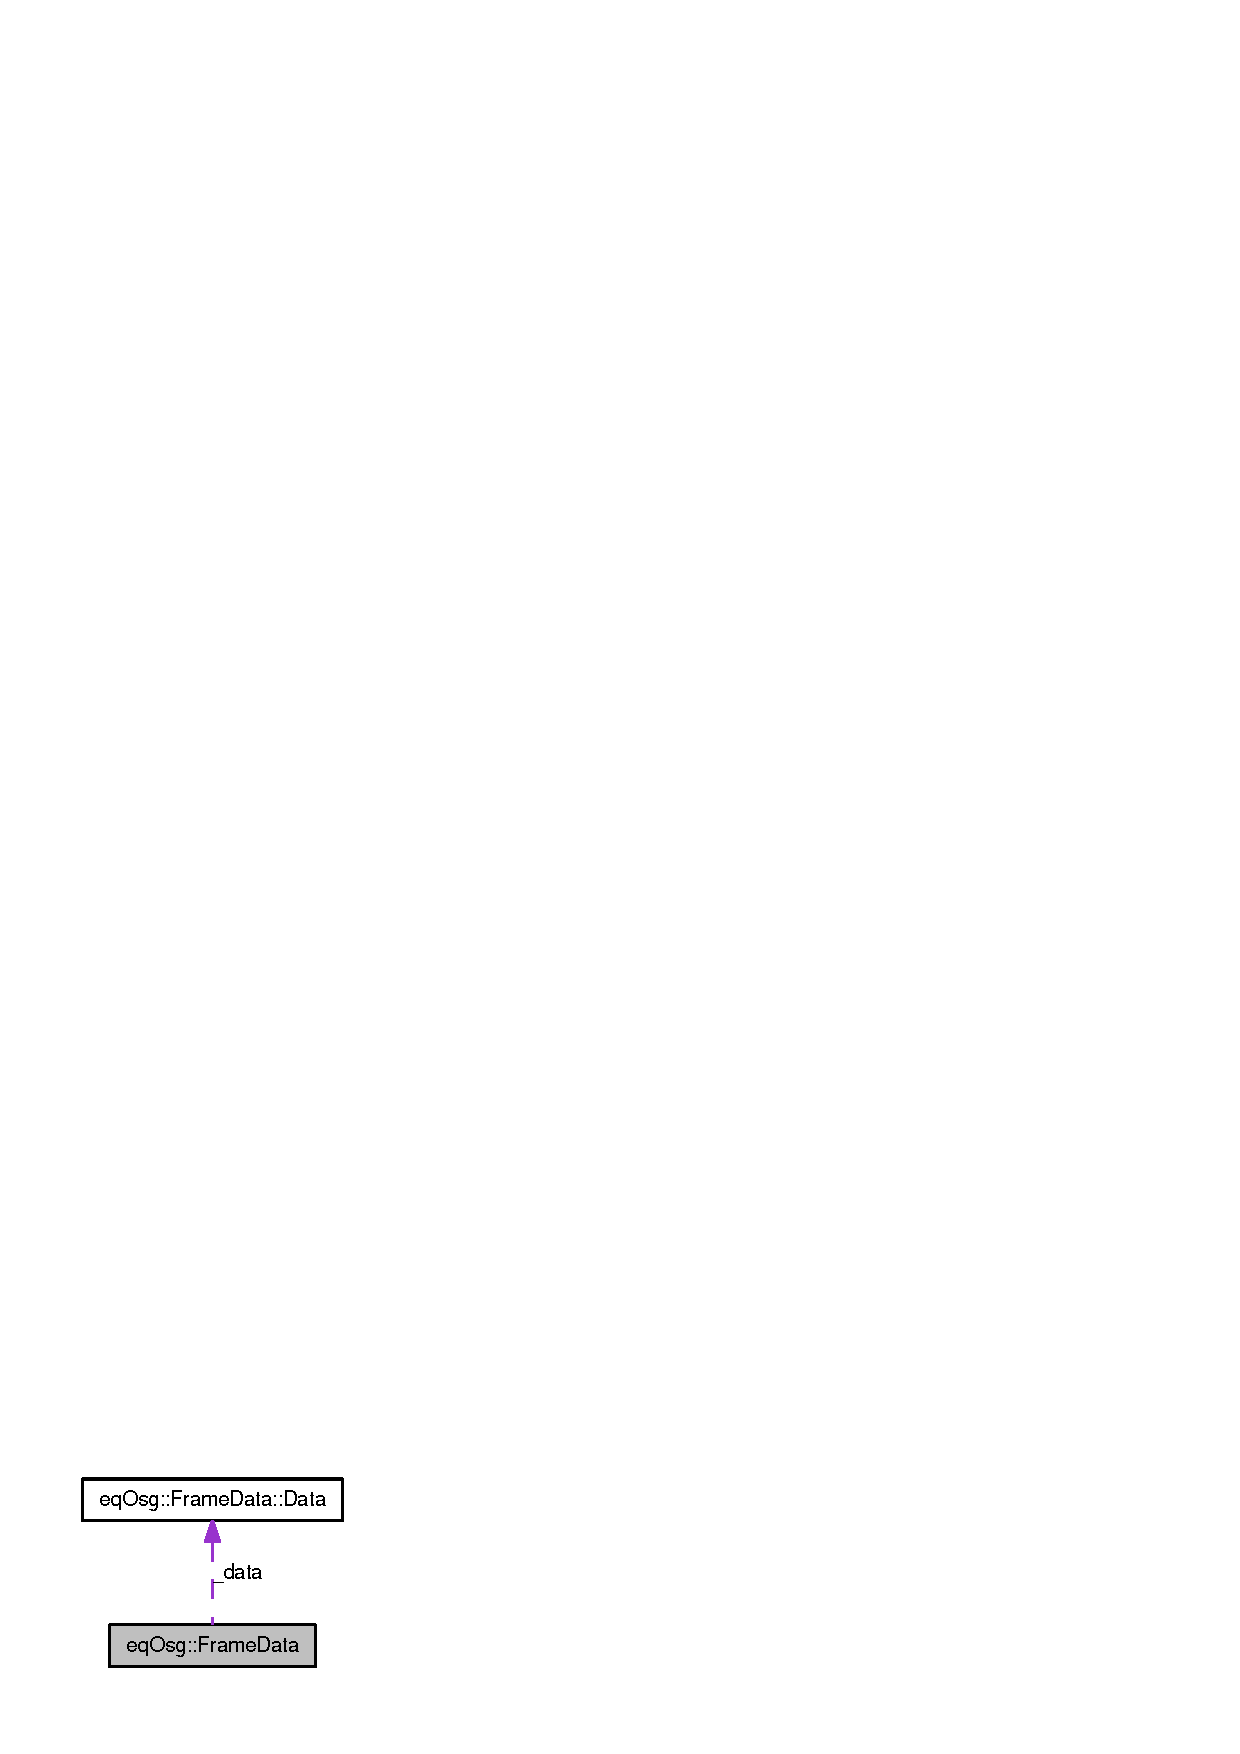
\includegraphics[width=168pt]{a00094}
\end{center}
\end{figure}
\subsection*{Classes}
\begin{CompactItemize}
\item 
struct \hyperlink{a00008}{Data}
\begin{CompactList}\small\item\em The FrameData's struct to hold members. \item\end{CompactList}\end{CompactItemize}
\subsection*{Public Member Functions}
\begin{CompactItemize}
\item 
\hyperlink{a00010_25212bee682363205562fae39028c3d6}{FrameData} ()
\begin{CompactList}\small\item\em Initialises everything to zero. \item\end{CompactList}\end{CompactItemize}
\subsection*{Public Attributes}
\begin{CompactItemize}
\item 
\hypertarget{a00010_bb269cc113e09a51c17d8d7400c6f1bb}{
\hyperlink{a00008}{Data} \hyperlink{a00010_bb269cc113e09a51c17d8d7400c6f1bb}{\_\-data}}
\label{a00010_bb269cc113e09a51c17d8d7400c6f1bb}

\begin{CompactList}\small\item\em our data struct \item\end{CompactList}\item 
\hypertarget{a00010_11589a99465896a1c632509c463c1577}{
std::vector$<$ eq::Event $>$ \hyperlink{a00010_11589a99465896a1c632509c463c1577}{\_\-eventQueue}}
\label{a00010_11589a99465896a1c632509c463c1577}

\begin{CompactList}\small\item\em save the eq events to pass it to the pipe \item\end{CompactList}\end{CompactItemize}
\subsection*{Protected Member Functions}
\begin{CompactItemize}
\item 
virtual eq::net::Object::ChangeType \hyperlink{a00010_00b26118522849f58fcc66b140a1c005}{getChangeType} () const 
\begin{CompactList}\small\item\em Change type is set to INSTANCE. \item\end{CompactList}\item 
virtual void \hyperlink{a00010_67d459f6a98840d88b1a0955aa4f517e}{getInstanceData} (eq::net::DataOStream \&stream)
\begin{CompactList}\small\item\em Passes the FrameData's data to the stream. \item\end{CompactList}\item 
virtual void \hyperlink{a00010_2dc720c76b371a3bd5edba7020808542}{applyInstanceData} (eq::net::DataIStream \&stream)
\begin{CompactList}\small\item\em Gets the data out of the stream. \item\end{CompactList}\end{CompactItemize}


\subsection{Detailed Description}
\hyperlink{a00010}{FrameData} holds all data which is updated each frame. 

It is sent by the server to all render clients. 

\subsection{Constructor \& Destructor Documentation}
\hypertarget{a00010_25212bee682363205562fae39028c3d6}{
\index{eqOsg::FrameData@{eqOsg::FrameData}!FrameData@{FrameData}}
\index{FrameData@{FrameData}!eqOsg::FrameData@{eqOsg::FrameData}}
\subsubsection[{FrameData}]{\setlength{\rightskip}{0pt plus 5cm}FrameData::FrameData ()}}
\label{a00010_25212bee682363205562fae39028c3d6}


Initialises everything to zero. 



camera base setup 

\subsection{Member Function Documentation}
\hypertarget{a00010_2dc720c76b371a3bd5edba7020808542}{
\index{eqOsg::FrameData@{eqOsg::FrameData}!applyInstanceData@{applyInstanceData}}
\index{applyInstanceData@{applyInstanceData}!eqOsg::FrameData@{eqOsg::FrameData}}
\subsubsection[{applyInstanceData}]{\setlength{\rightskip}{0pt plus 5cm}void FrameData::applyInstanceData (eq::net::DataIStream \& {\em stream})\hspace{0.3cm}{\tt  \mbox{[}protected, virtual\mbox{]}}}}
\label{a00010_2dc720c76b371a3bd5edba7020808542}


Gets the data out of the stream. 

\begin{Desc}
\item[Parameters:]
\begin{description}
\item[{\em stream}]The Equalizer stream to read. \end{description}
\end{Desc}


get the framedata out of the stream \hypertarget{a00010_00b26118522849f58fcc66b140a1c005}{
\index{eqOsg::FrameData@{eqOsg::FrameData}!getChangeType@{getChangeType}}
\index{getChangeType@{getChangeType}!eqOsg::FrameData@{eqOsg::FrameData}}
\subsubsection[{getChangeType}]{\setlength{\rightskip}{0pt plus 5cm}eq::net::Object::ChangeType FrameData::getChangeType () const\hspace{0.3cm}{\tt  \mbox{[}protected, virtual\mbox{]}}}}
\label{a00010_00b26118522849f58fcc66b140a1c005}


Change type is set to INSTANCE. 

\begin{Desc}
\item[Returns:]The Equalizer change type. \end{Desc}
\hypertarget{a00010_67d459f6a98840d88b1a0955aa4f517e}{
\index{eqOsg::FrameData@{eqOsg::FrameData}!getInstanceData@{getInstanceData}}
\index{getInstanceData@{getInstanceData}!eqOsg::FrameData@{eqOsg::FrameData}}
\subsubsection[{getInstanceData}]{\setlength{\rightskip}{0pt plus 5cm}void FrameData::getInstanceData (eq::net::DataOStream \& {\em stream})\hspace{0.3cm}{\tt  \mbox{[}protected, virtual\mbox{]}}}}
\label{a00010_67d459f6a98840d88b1a0955aa4f517e}


Passes the FrameData's data to the stream. 

\begin{Desc}
\item[Parameters:]
\begin{description}
\item[{\em stream}]The Equalizer stream to write. \end{description}
\end{Desc}


write the framedata to the stream 

The documentation for this class was generated from the following files:\begin{CompactItemize}
\item 
E:/schule/Thesis/Repo/trunk/crf/src/FrameData.h\item 
E:/schule/Thesis/Repo/trunk/crf/src/FrameData.cpp\end{CompactItemize}

\hypertarget{a00011}{
\section{eqOsg::InitData Class Reference}
\label{a00011}\index{eqOsg::InitData@{eqOsg::InitData}}
}
The init data holds all data which is needed during initalization.  


{\tt \#include $<$InitData.h$>$}

\subsection*{Public Member Functions}
\begin{CompactItemize}
\item 
\hypertarget{a00011_9186b2f084ea9016e1bd8f5c98ccb55e}{
\hyperlink{a00011_9186b2f084ea9016e1bd8f5c98ccb55e}{$\sim$InitData} ()}
\label{a00011_9186b2f084ea9016e1bd8f5c98ccb55e}

\begin{CompactList}\small\item\em \hyperlink{a00011}{InitData} deconstructor. \item\end{CompactList}\item 
void \hyperlink{a00011_784dbe6a89945a5311143ca91b01c224}{setFrameDataID} (const uint32\_\-t id)
\begin{CompactList}\small\item\em Sets the frame ID. \item\end{CompactList}\item 
uint32\_\-t \hyperlink{a00011_0fed75d0be3cc9d30aa2483920dda8ec}{getFrameDataID} () const 
\begin{CompactList}\small\item\em Returns the frame ID. \item\end{CompactList}\item 
bool \hyperlink{a00011_911e15d0bc1d4e427ad574a9b9e0fff9}{parseCommandLine} (char $\ast$$\ast$argv, int argc)
\begin{CompactList}\small\item\em Parses the command line arguments and puts the things it can parse into the init data. \item\end{CompactList}\item 
void \hyperlink{a00011_de8e662e01371948b9717ffe8412ed45}{setLoadModel} (bool loadModel)
\begin{CompactList}\small\item\em Should an osg file model be loaded? This is usually set by \hyperlink{a00011_911e15d0bc1d4e427ad574a9b9e0fff9}{InitData::parseCommandLine()}. \item\end{CompactList}\item 
bool \hyperlink{a00011_98db3359b5152eebe9967b0e4cf3e29a}{getLoadModel} () const 
\begin{CompactList}\small\item\em Should an osg file model be loaded? This is usually set by \hyperlink{a00011_911e15d0bc1d4e427ad574a9b9e0fff9}{InitData::parseCommandLine()}. \item\end{CompactList}\item 
void \hyperlink{a00011_71d9d6c19244b8bf10e8fae264a2327c}{setModelFileName} (const std::string \&fileName)
\begin{CompactList}\small\item\em Sets the to load model file name. \item\end{CompactList}\item 
std::string \hyperlink{a00011_b5f311698f1dd969d0a968fb06929426}{getModelFileName} () const 
\begin{CompactList}\small\item\em Returns the model filename. \item\end{CompactList}\end{CompactItemize}
\subsection*{Protected Member Functions}
\begin{CompactItemize}
\item 
virtual void \hyperlink{a00011_3604e3e7cc5b5c19f62bcf44d75d459f}{getInstanceData} (eq::net::DataOStream \&stream)
\begin{CompactList}\small\item\em Passes the InitData's data to the stream. \item\end{CompactList}\item 
virtual void \hyperlink{a00011_c9fa7b403a16477dc402a2e31b04ca50}{applyInstanceData} (eq::net::DataIStream \&stream)
\begin{CompactList}\small\item\em Gets the data out of the stream. \item\end{CompactList}\end{CompactItemize}


\subsection{Detailed Description}
The init data holds all data which is needed during initalization. 

It is sent by the server to all render clients. It holds the frame data ID, so all clients can sync the frame data object. 

\subsection{Member Function Documentation}
\hypertarget{a00011_c9fa7b403a16477dc402a2e31b04ca50}{
\index{eqOsg::InitData@{eqOsg::InitData}!applyInstanceData@{applyInstanceData}}
\index{applyInstanceData@{applyInstanceData}!eqOsg::InitData@{eqOsg::InitData}}
\subsubsection[{applyInstanceData}]{\setlength{\rightskip}{0pt plus 5cm}void InitData::applyInstanceData (eq::net::DataIStream \& {\em stream})\hspace{0.3cm}{\tt  \mbox{[}protected, virtual\mbox{]}}}}
\label{a00011_c9fa7b403a16477dc402a2e31b04ca50}


Gets the data out of the stream. 

\begin{Desc}
\item[Parameters:]
\begin{description}
\item[{\em stream}]The Equalizer stream to read. \end{description}
\end{Desc}
\hypertarget{a00011_0fed75d0be3cc9d30aa2483920dda8ec}{
\index{eqOsg::InitData@{eqOsg::InitData}!getFrameDataID@{getFrameDataID}}
\index{getFrameDataID@{getFrameDataID}!eqOsg::InitData@{eqOsg::InitData}}
\subsubsection[{getFrameDataID}]{\setlength{\rightskip}{0pt plus 5cm}uint32\_\-t InitData::getFrameDataID () const}}
\label{a00011_0fed75d0be3cc9d30aa2483920dda8ec}


Returns the frame ID. 

\begin{Desc}
\item[Returns:]The ID. \end{Desc}
\hypertarget{a00011_3604e3e7cc5b5c19f62bcf44d75d459f}{
\index{eqOsg::InitData@{eqOsg::InitData}!getInstanceData@{getInstanceData}}
\index{getInstanceData@{getInstanceData}!eqOsg::InitData@{eqOsg::InitData}}
\subsubsection[{getInstanceData}]{\setlength{\rightskip}{0pt plus 5cm}void InitData::getInstanceData (eq::net::DataOStream \& {\em stream})\hspace{0.3cm}{\tt  \mbox{[}protected, virtual\mbox{]}}}}
\label{a00011_3604e3e7cc5b5c19f62bcf44d75d459f}


Passes the InitData's data to the stream. 

\begin{Desc}
\item[Parameters:]
\begin{description}
\item[{\em stream}]The Equalizer stream to write. \end{description}
\end{Desc}
\hypertarget{a00011_98db3359b5152eebe9967b0e4cf3e29a}{
\index{eqOsg::InitData@{eqOsg::InitData}!getLoadModel@{getLoadModel}}
\index{getLoadModel@{getLoadModel}!eqOsg::InitData@{eqOsg::InitData}}
\subsubsection[{getLoadModel}]{\setlength{\rightskip}{0pt plus 5cm}bool eqOsg::InitData::getLoadModel () const\hspace{0.3cm}{\tt  \mbox{[}inline\mbox{]}}}}
\label{a00011_98db3359b5152eebe9967b0e4cf3e29a}


Should an osg file model be loaded? This is usually set by \hyperlink{a00011_911e15d0bc1d4e427ad574a9b9e0fff9}{InitData::parseCommandLine()}. 

\begin{Desc}
\item[Returns:]True if a model will be loaded by the pipe. \end{Desc}
\hypertarget{a00011_b5f311698f1dd969d0a968fb06929426}{
\index{eqOsg::InitData@{eqOsg::InitData}!getModelFileName@{getModelFileName}}
\index{getModelFileName@{getModelFileName}!eqOsg::InitData@{eqOsg::InitData}}
\subsubsection[{getModelFileName}]{\setlength{\rightskip}{0pt plus 5cm}std::string eqOsg::InitData::getModelFileName () const\hspace{0.3cm}{\tt  \mbox{[}inline\mbox{]}}}}
\label{a00011_b5f311698f1dd969d0a968fb06929426}


Returns the model filename. 

\begin{Desc}
\item[Returns:]The filename of the to load model. \end{Desc}
\hypertarget{a00011_911e15d0bc1d4e427ad574a9b9e0fff9}{
\index{eqOsg::InitData@{eqOsg::InitData}!parseCommandLine@{parseCommandLine}}
\index{parseCommandLine@{parseCommandLine}!eqOsg::InitData@{eqOsg::InitData}}
\subsubsection[{parseCommandLine}]{\setlength{\rightskip}{0pt plus 5cm}bool InitData::parseCommandLine (char $\ast$$\ast$ {\em argv}, \/  int {\em argc})}}
\label{a00011_911e15d0bc1d4e427ad574a9b9e0fff9}


Parses the command line arguments and puts the things it can parse into the init data. 

\begin{Desc}
\item[Parameters:]
\begin{description}
\item[{\em argv}]The passed arguments. \item[{\em argc}]The passed arguments' counter. \end{description}
\end{Desc}
\begin{Desc}
\item[Returns:]true if the command line was successfully parsed, false otherwise. \end{Desc}
\hypertarget{a00011_784dbe6a89945a5311143ca91b01c224}{
\index{eqOsg::InitData@{eqOsg::InitData}!setFrameDataID@{setFrameDataID}}
\index{setFrameDataID@{setFrameDataID}!eqOsg::InitData@{eqOsg::InitData}}
\subsubsection[{setFrameDataID}]{\setlength{\rightskip}{0pt plus 5cm}void InitData::setFrameDataID (const uint32\_\-t {\em id})}}
\label{a00011_784dbe6a89945a5311143ca91b01c224}


Sets the frame ID. 

\begin{Desc}
\item[Parameters:]
\begin{description}
\item[{\em id}]The id of the frame. \end{description}
\end{Desc}
\hypertarget{a00011_de8e662e01371948b9717ffe8412ed45}{
\index{eqOsg::InitData@{eqOsg::InitData}!setLoadModel@{setLoadModel}}
\index{setLoadModel@{setLoadModel}!eqOsg::InitData@{eqOsg::InitData}}
\subsubsection[{setLoadModel}]{\setlength{\rightskip}{0pt plus 5cm}void eqOsg::InitData::setLoadModel (bool {\em loadModel})\hspace{0.3cm}{\tt  \mbox{[}inline\mbox{]}}}}
\label{a00011_de8e662e01371948b9717ffe8412ed45}


Should an osg file model be loaded? This is usually set by \hyperlink{a00011_911e15d0bc1d4e427ad574a9b9e0fff9}{InitData::parseCommandLine()}. 

\begin{Desc}
\item[Parameters:]
\begin{description}
\item[{\em loadModel}]True/False \end{description}
\end{Desc}
\hypertarget{a00011_71d9d6c19244b8bf10e8fae264a2327c}{
\index{eqOsg::InitData@{eqOsg::InitData}!setModelFileName@{setModelFileName}}
\index{setModelFileName@{setModelFileName}!eqOsg::InitData@{eqOsg::InitData}}
\subsubsection[{setModelFileName}]{\setlength{\rightskip}{0pt plus 5cm}void eqOsg::InitData::setModelFileName (const std::string \& {\em fileName})\hspace{0.3cm}{\tt  \mbox{[}inline\mbox{]}}}}
\label{a00011_71d9d6c19244b8bf10e8fae264a2327c}


Sets the to load model file name. 

\begin{Desc}
\item[Parameters:]
\begin{description}
\item[{\em fileName}]An existing osg model in the filesystem. \end{description}
\end{Desc}


The documentation for this class was generated from the following files:\begin{CompactItemize}
\item 
E:/schule/Thesis/Repo/trunk/crf/src/InitData.h\item 
E:/schule/Thesis/Repo/trunk/crf/src/InitData.cpp\end{CompactItemize}

\hypertarget{a00012}{
\section{eqOsg::Node Class Reference}
\label{a00012}\index{eqOsg::Node@{eqOsg::Node}}
}
A node represents the renderclient.  


{\tt \#include $<$Node.h$>$}

\subsection*{Public Member Functions}
\begin{CompactItemize}
\item 
\hyperlink{a00012_31378a45a15dd93ae53ec380c54c1ded}{Node} (eq::Config $\ast$parent)
\end{CompactItemize}
\subsection*{Protected Member Functions}
\begin{CompactItemize}
\item 
virtual bool \hyperlink{a00012_ba19d8a715644e09e7c5490ff1932659}{configInit} (const uint32\_\-t initID)
\begin{CompactList}\small\item\em Generates \char`\"{}our\char`\"{} ConfigInit object. \item\end{CompactList}\end{CompactItemize}


\subsection{Detailed Description}
A node represents the renderclient. 

because this part doesn't bother the std-equalizer implementation, we don't need big changes here \begin{Desc}
\item[See also:]eq::Node \end{Desc}


\subsection{Constructor \& Destructor Documentation}
\hypertarget{a00012_31378a45a15dd93ae53ec380c54c1ded}{
\index{eqOsg::Node@{eqOsg::Node}!Node@{Node}}
\index{Node@{Node}!eqOsg::Node@{eqOsg::Node}}
\subsubsection[{Node}]{\setlength{\rightskip}{0pt plus 5cm}Node::Node (eq::Config $\ast$ {\em parent})}}
\label{a00012_31378a45a15dd93ae53ec380c54c1ded}


\begin{Desc}
\item[See also:]eq::Node::Node \end{Desc}


\subsection{Member Function Documentation}
\hypertarget{a00012_ba19d8a715644e09e7c5490ff1932659}{
\index{eqOsg::Node@{eqOsg::Node}!configInit@{configInit}}
\index{configInit@{configInit}!eqOsg::Node@{eqOsg::Node}}
\subsubsection[{configInit}]{\setlength{\rightskip}{0pt plus 5cm}bool Node::configInit (const uint32\_\-t {\em initID})\hspace{0.3cm}{\tt  \mbox{[}protected, virtual\mbox{]}}}}
\label{a00012_ba19d8a715644e09e7c5490ff1932659}


Generates \char`\"{}our\char`\"{} ConfigInit object. 

\begin{Desc}
\item[Parameters:]
\begin{description}
\item[{\em initID}]The initID. \end{description}
\end{Desc}


The documentation for this class was generated from the following files:\begin{CompactItemize}
\item 
E:/schule/Thesis/Repo/trunk/crf/src/Node.h\item 
E:/schule/Thesis/Repo/trunk/crf/src/Node.cpp\end{CompactItemize}

\hypertarget{a00013}{
\section{eqOsg::NodeFactory Class Reference}
\label{a00013}\index{eqOsg::NodeFactory@{eqOsg::NodeFactory}}
}
Our eq node factory to create the \hyperlink{a00045}{eqOsg} objects.  


{\tt \#include $<$NodeFactory.h$>$}

Inherited by \hyperlink{a00005}{crf::crfNodeFactory}.

\subsection*{Public Member Functions}
\begin{CompactItemize}
\item 
virtual eq::Channel $\ast$ \hyperlink{a00013_9cd8a51ad40a04fae74c86d20c5ad561}{createChannel} (eq::Window $\ast$parent)
\begin{CompactList}\small\item\em creates the \hyperlink{a00002}{eqOsg::Channel} object \item\end{CompactList}\item 
virtual eq::Config $\ast$ \hyperlink{a00013_0e80614084de6b23a4a2677fc8af7f93}{createConfig} (eq::ServerPtr parent)
\begin{CompactList}\small\item\em creates the \hyperlink{a00003}{eqOsg::Config} object \item\end{CompactList}\item 
virtual eq::Node $\ast$ \hyperlink{a00013_9a411368eca08325cdc5f80ea687f217}{createNode} (eq::Config $\ast$parent)
\begin{CompactList}\small\item\em creates the \hyperlink{a00012}{eqOsg::Node} object \item\end{CompactList}\item 
virtual eq::Pipe $\ast$ \hyperlink{a00013_10e06f5d0d32f146994274682d39e666}{createPipe} (eq::Node $\ast$parent)
\begin{CompactList}\small\item\em creates the \hyperlink{a00014}{eqOsg::Pipe} object \item\end{CompactList}\end{CompactItemize}


\subsection{Detailed Description}
Our eq node factory to create the \hyperlink{a00045}{eqOsg} objects. 

If you create your own objects, this factory has to be overriden and passed when calling eq::init. \begin{Desc}
\item[See also:]eq::NodeFactory \end{Desc}


\subsection{Member Function Documentation}
\hypertarget{a00013_9cd8a51ad40a04fae74c86d20c5ad561}{
\index{eqOsg::NodeFactory@{eqOsg::NodeFactory}!createChannel@{createChannel}}
\index{createChannel@{createChannel}!eqOsg::NodeFactory@{eqOsg::NodeFactory}}
\subsubsection[{createChannel}]{\setlength{\rightskip}{0pt plus 5cm}virtual eq::Channel$\ast$ eqOsg::NodeFactory::createChannel (eq::Window $\ast$ {\em parent})\hspace{0.3cm}{\tt  \mbox{[}inline, virtual\mbox{]}}}}
\label{a00013_9cd8a51ad40a04fae74c86d20c5ad561}


creates the \hyperlink{a00002}{eqOsg::Channel} object 

\begin{Desc}
\item[Parameters:]
\begin{description}
\item[{\em parent}]The channel's parent window. \end{description}
\end{Desc}
\begin{Desc}
\item[Returns:]The \hyperlink{a00002}{eqOsg::Channel}. \end{Desc}
\hypertarget{a00013_0e80614084de6b23a4a2677fc8af7f93}{
\index{eqOsg::NodeFactory@{eqOsg::NodeFactory}!createConfig@{createConfig}}
\index{createConfig@{createConfig}!eqOsg::NodeFactory@{eqOsg::NodeFactory}}
\subsubsection[{createConfig}]{\setlength{\rightskip}{0pt plus 5cm}virtual eq::Config$\ast$ eqOsg::NodeFactory::createConfig (eq::ServerPtr {\em parent})\hspace{0.3cm}{\tt  \mbox{[}inline, virtual\mbox{]}}}}
\label{a00013_0e80614084de6b23a4a2677fc8af7f93}


creates the \hyperlink{a00003}{eqOsg::Config} object 

\begin{Desc}
\item[Parameters:]
\begin{description}
\item[{\em parent}]The config's parent server. \end{description}
\end{Desc}
\begin{Desc}
\item[Returns:]The \hyperlink{a00003}{eqOsg::Config}. \end{Desc}


Reimplemented in \hyperlink{a00005_0b7b562ae3d0ccc5a98017195926057f}{crf::crfNodeFactory}.\hypertarget{a00013_9a411368eca08325cdc5f80ea687f217}{
\index{eqOsg::NodeFactory@{eqOsg::NodeFactory}!createNode@{createNode}}
\index{createNode@{createNode}!eqOsg::NodeFactory@{eqOsg::NodeFactory}}
\subsubsection[{createNode}]{\setlength{\rightskip}{0pt plus 5cm}virtual eq::Node$\ast$ eqOsg::NodeFactory::createNode (eq::Config $\ast$ {\em parent})\hspace{0.3cm}{\tt  \mbox{[}inline, virtual\mbox{]}}}}
\label{a00013_9a411368eca08325cdc5f80ea687f217}


creates the \hyperlink{a00012}{eqOsg::Node} object 

\begin{Desc}
\item[Parameters:]
\begin{description}
\item[{\em parent}]The node's parent config. \end{description}
\end{Desc}
\begin{Desc}
\item[Returns:]The \hyperlink{a00012}{eqOsg::Node}. \end{Desc}
\hypertarget{a00013_10e06f5d0d32f146994274682d39e666}{
\index{eqOsg::NodeFactory@{eqOsg::NodeFactory}!createPipe@{createPipe}}
\index{createPipe@{createPipe}!eqOsg::NodeFactory@{eqOsg::NodeFactory}}
\subsubsection[{createPipe}]{\setlength{\rightskip}{0pt plus 5cm}virtual eq::Pipe$\ast$ eqOsg::NodeFactory::createPipe (eq::Node $\ast$ {\em parent})\hspace{0.3cm}{\tt  \mbox{[}inline, virtual\mbox{]}}}}
\label{a00013_10e06f5d0d32f146994274682d39e666}


creates the \hyperlink{a00014}{eqOsg::Pipe} object 

\begin{Desc}
\item[Parameters:]
\begin{description}
\item[{\em parent}]The pipe's parent node. \end{description}
\end{Desc}
\begin{Desc}
\item[Returns:]The \hyperlink{a00014}{eqOsg::Pipe}. \end{Desc}


Reimplemented in \hyperlink{a00005_5f35c307f323b385869226c6083df93d}{crf::crfNodeFactory}.

The documentation for this class was generated from the following file:\begin{CompactItemize}
\item 
E:/schule/Thesis/Repo/trunk/crf/src/NodeFactory.h\end{CompactItemize}

\hypertarget{a00014}{
\section{eqOsg::Pipe Class Reference}
\label{a00014}\index{eqOsg::Pipe@{eqOsg::Pipe}}
}
The \hyperlink{a00014}{Pipe} holds the viewer and the frame data.  


{\tt \#include $<$Pipe.h$>$}

Inherited by \hyperlink{a00006}{crf::crfPipe}.

Collaboration diagram for eqOsg::Pipe:\nopagebreak
\begin{figure}[H]
\begin{center}
\leavevmode
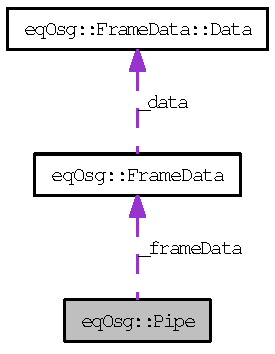
\includegraphics[width=168pt]{a00101}
\end{center}
\end{figure}
\subsection*{Public Member Functions}
\begin{CompactItemize}
\item 
\hyperlink{a00014_70ba41100439b9cd50a7aeea8060d5ac}{Pipe} (eq::Node $\ast$parent)
\item 
const \hyperlink{a00010}{FrameData} \& \hyperlink{a00014_b0c77c44b8b387666ef45b76bc8d2284}{getFrameData} () const 
\begin{CompactList}\small\item\em Returns the pipe's \hyperlink{a00010}{FrameData} object. \item\end{CompactList}\item 
osg::ref\_\-ptr$<$ \hyperlink{a00009}{eqOsg::EqViewer} $>$ \hyperlink{a00014_e0cf2ae4fae2e59cbb65374084c8b563}{getViewer} () const 
\begin{CompactList}\small\item\em Returns the pipe's \hyperlink{a00009}{EqViewer}. \item\end{CompactList}\end{CompactItemize}
\subsection*{Protected Member Functions}
\begin{CompactItemize}
\item 
virtual bool \hyperlink{a00014_d23bd6f7bb0f59f94fc0e279dbbb9d9a}{configInit} (const uint32\_\-t initID)
\begin{CompactList}\small\item\em Registers the frame data, so it can be synced with the server later. \item\end{CompactList}\item 
virtual bool \hyperlink{a00014_2cb47387a7be185b1dc6d097dc4da38e}{configExit} ()
\begin{CompactList}\small\item\em Deregisters the frame data. \item\end{CompactList}\item 
virtual void \hyperlink{a00014_6be431b1b9fe04da31596ea8b870dfde}{frameStart} (const uint32\_\-t frameID, const uint32\_\-t frameNumber)
\begin{CompactList}\small\item\em Syncs the frame data with the server and calls updateSceneGraph(). \item\end{CompactList}\item 
virtual void \hyperlink{a00014_bb1e29569fab6e079fc1fcb286af4f40}{createSceneGraph} (std::string modelFileName)
\begin{CompactList}\small\item\em Creates a scene graph with a model by filename. \item\end{CompactList}\item 
virtual osg::ref\_\-ptr$<$ osg::Node $>$ \hyperlink{a00014_b357cd9e8e214f839388de82e14333a1}{correctCoordsys} (osg::ref\_\-ptr$<$ osg::Node $>$ nodeToRotate)
\begin{CompactList}\small\item\em Corrects the coordination system from osg to eq. \item\end{CompactList}\item 
osg::ref\_\-ptr$<$ osg::Node $>$ \hyperlink{a00014_7f42242765d3cb5b0132bfc5c8ed7142}{correctCoordsys} (osg::ref\_\-ptr$<$ osg::Node $>$ nodeToTransform, osg::Matrix matrix)
\begin{CompactList}\small\item\em Transform a desired node around a passed matrix. \item\end{CompactList}\end{CompactItemize}
\subsection*{Protected Attributes}
\begin{CompactItemize}
\item 
\hypertarget{a00014_b4f8193b938ef155c87df88e084e42fc}{
\hyperlink{a00010}{FrameData} \hyperlink{a00014_b4f8193b938ef155c87df88e084e42fc}{\_\-frameData}}
\label{a00014_b4f8193b938ef155c87df88e084e42fc}

\begin{CompactList}\small\item\em The \hyperlink{a00010}{FrameData} object. \item\end{CompactList}\item 
\hypertarget{a00014_e36ebe17666eeda7d5293077a69ba6ad}{
osg::ref\_\-ptr$<$ \hyperlink{a00009}{eqOsg::EqViewer} $>$ \hyperlink{a00014_e36ebe17666eeda7d5293077a69ba6ad}{\_\-viewer}}
\label{a00014_e36ebe17666eeda7d5293077a69ba6ad}

\begin{CompactList}\small\item\em The pipe's \hyperlink{a00009}{EqViewer}. \item\end{CompactList}\item 
\hypertarget{a00014_c58577ad857d962e3f4da22492911631}{
bool \hyperlink{a00014_c58577ad857d962e3f4da22492911631}{\_\-sceneGraphCreated}}
\label{a00014_c58577ad857d962e3f4da22492911631}

\begin{CompactList}\small\item\em Set to true if the scene graph has been created and added to the viewer. \item\end{CompactList}\item 
\hypertarget{a00014_ac2035c8102ec6a66160453963b1d9b4}{
bool \hyperlink{a00014_ac2035c8102ec6a66160453963b1d9b4}{\_\-usesModel}}
\label{a00014_ac2035c8102ec6a66160453963b1d9b4}

\begin{CompactList}\small\item\em Set to true if a simple model shoudl be load. \item\end{CompactList}\item 
\hypertarget{a00014_4cc32263a7c4cb68639f65bc7a18ca49}{
std::string \hyperlink{a00014_4cc32263a7c4cb68639f65bc7a18ca49}{\_\-modelFile}}
\label{a00014_4cc32263a7c4cb68639f65bc7a18ca49}

\begin{CompactList}\small\item\em The filename of the to-load model. \item\end{CompactList}\end{CompactItemize}


\subsection{Detailed Description}
The \hyperlink{a00014}{Pipe} holds the viewer and the frame data. 

Each frame, it updates the scene graph of the viewer with the new data of the frame data. The frame data is synced with the server. \begin{Desc}
\item[See also:]eq::Pipe \end{Desc}


\subsection{Constructor \& Destructor Documentation}
\hypertarget{a00014_70ba41100439b9cd50a7aeea8060d5ac}{
\index{eqOsg::Pipe@{eqOsg::Pipe}!Pipe@{Pipe}}
\index{Pipe@{Pipe}!eqOsg::Pipe@{eqOsg::Pipe}}
\subsubsection[{Pipe}]{\setlength{\rightskip}{0pt plus 5cm}Pipe::Pipe (eq::Node $\ast$ {\em parent})}}
\label{a00014_70ba41100439b9cd50a7aeea8060d5ac}


\begin{Desc}
\item[See also:]eq::Pipe::Pipe \end{Desc}


\subsection{Member Function Documentation}
\hypertarget{a00014_2cb47387a7be185b1dc6d097dc4da38e}{
\index{eqOsg::Pipe@{eqOsg::Pipe}!configExit@{configExit}}
\index{configExit@{configExit}!eqOsg::Pipe@{eqOsg::Pipe}}
\subsubsection[{configExit}]{\setlength{\rightskip}{0pt plus 5cm}bool Pipe::configExit ()\hspace{0.3cm}{\tt  \mbox{[}protected, virtual\mbox{]}}}}
\label{a00014_2cb47387a7be185b1dc6d097dc4da38e}


Deregisters the frame data. 

\begin{Desc}
\item[Returns:]True if everything worked fine. \end{Desc}


Reimplemented in \hyperlink{a00006_3f48f5f5a8a455342b111f26ca1402db}{crf::crfPipe}.\hypertarget{a00014_d23bd6f7bb0f59f94fc0e279dbbb9d9a}{
\index{eqOsg::Pipe@{eqOsg::Pipe}!configInit@{configInit}}
\index{configInit@{configInit}!eqOsg::Pipe@{eqOsg::Pipe}}
\subsubsection[{configInit}]{\setlength{\rightskip}{0pt plus 5cm}bool Pipe::configInit (const uint32\_\-t {\em initID})\hspace{0.3cm}{\tt  \mbox{[}protected, virtual\mbox{]}}}}
\label{a00014_d23bd6f7bb0f59f94fc0e279dbbb9d9a}


Registers the frame data, so it can be synced with the server later. 

\begin{Desc}
\item[Parameters:]
\begin{description}
\item[{\em initID}]The Equalizer initID. \end{description}
\end{Desc}
\begin{Desc}
\item[Returns:]True if everything worked fine. \end{Desc}


Reimplemented in \hyperlink{a00006_fcf11863d5370a815bd7e1216cc0f2e6}{crf::crfPipe}.\hypertarget{a00014_7f42242765d3cb5b0132bfc5c8ed7142}{
\index{eqOsg::Pipe@{eqOsg::Pipe}!correctCoordsys@{correctCoordsys}}
\index{correctCoordsys@{correctCoordsys}!eqOsg::Pipe@{eqOsg::Pipe}}
\subsubsection[{correctCoordsys}]{\setlength{\rightskip}{0pt plus 5cm}osg::ref\_\-ptr$<$ osg::Node $>$ Pipe::correctCoordsys (osg::ref\_\-ptr$<$ osg::Node $>$ {\em nodeToTransform}, \/  osg::Matrix {\em matrix})\hspace{0.3cm}{\tt  \mbox{[}protected\mbox{]}}}}
\label{a00014_7f42242765d3cb5b0132bfc5c8ed7142}


Transform a desired node around a passed matrix. 

\begin{Desc}
\item[Parameters:]
\begin{description}
\item[{\em nodeToTransform}]The node, which should be transformed. \item[{\em matrix}]The transformation matrix. \end{description}
\end{Desc}
\begin{Desc}
\item[Returns:]The transformed node. \end{Desc}
\hypertarget{a00014_b357cd9e8e214f839388de82e14333a1}{
\index{eqOsg::Pipe@{eqOsg::Pipe}!correctCoordsys@{correctCoordsys}}
\index{correctCoordsys@{correctCoordsys}!eqOsg::Pipe@{eqOsg::Pipe}}
\subsubsection[{correctCoordsys}]{\setlength{\rightskip}{0pt plus 5cm}osg::ref\_\-ptr$<$ osg::Node $>$ Pipe::correctCoordsys (osg::ref\_\-ptr$<$ osg::Node $>$ {\em nodeToRotate})\hspace{0.3cm}{\tt  \mbox{[}protected, virtual\mbox{]}}}}
\label{a00014_b357cd9e8e214f839388de82e14333a1}


Corrects the coordination system from osg to eq. 

Rotates the whole scene 90� around the X-axis and 180 around Y to fit the commonly used Equalizer schema. \begin{Desc}
\item[Parameters:]
\begin{description}
\item[{\em nodeToRotate}]The node, which should be rotated \end{description}
\end{Desc}
\begin{Desc}
\item[Returns:]The rotated node \end{Desc}
\hypertarget{a00014_bb1e29569fab6e079fc1fcb286af4f40}{
\index{eqOsg::Pipe@{eqOsg::Pipe}!createSceneGraph@{createSceneGraph}}
\index{createSceneGraph@{createSceneGraph}!eqOsg::Pipe@{eqOsg::Pipe}}
\subsubsection[{createSceneGraph}]{\setlength{\rightskip}{0pt plus 5cm}void Pipe::createSceneGraph (std::string {\em modelFileName})\hspace{0.3cm}{\tt  \mbox{[}protected, virtual\mbox{]}}}}
\label{a00014_bb1e29569fab6e079fc1fcb286af4f40}


Creates a scene graph with a model by filename. 

\begin{Desc}
\item[Parameters:]
\begin{description}
\item[{\em modelFileName}]The filename of the model. \end{description}
\end{Desc}
\hypertarget{a00014_6be431b1b9fe04da31596ea8b870dfde}{
\index{eqOsg::Pipe@{eqOsg::Pipe}!frameStart@{frameStart}}
\index{frameStart@{frameStart}!eqOsg::Pipe@{eqOsg::Pipe}}
\subsubsection[{frameStart}]{\setlength{\rightskip}{0pt plus 5cm}void Pipe::frameStart (const uint32\_\-t {\em frameID}, \/  const uint32\_\-t {\em frameNumber})\hspace{0.3cm}{\tt  \mbox{[}protected, virtual\mbox{]}}}}
\label{a00014_6be431b1b9fe04da31596ea8b870dfde}


Syncs the frame data with the server and calls updateSceneGraph(). 

\begin{Desc}
\item[See also:]eq::Pipe::frameStart \end{Desc}


Reimplemented in \hyperlink{a00006_2e551fe08841da2b7a1def541656d48c}{crf::crfPipe}.\hypertarget{a00014_b0c77c44b8b387666ef45b76bc8d2284}{
\index{eqOsg::Pipe@{eqOsg::Pipe}!getFrameData@{getFrameData}}
\index{getFrameData@{getFrameData}!eqOsg::Pipe@{eqOsg::Pipe}}
\subsubsection[{getFrameData}]{\setlength{\rightskip}{0pt plus 5cm}const {\bf FrameData} \& Pipe::getFrameData () const}}
\label{a00014_b0c77c44b8b387666ef45b76bc8d2284}


Returns the pipe's \hyperlink{a00010}{FrameData} object. 

\begin{Desc}
\item[Returns:]The \hyperlink{a00010}{FrameData} of this pipe. \end{Desc}
\hypertarget{a00014_e0cf2ae4fae2e59cbb65374084c8b563}{
\index{eqOsg::Pipe@{eqOsg::Pipe}!getViewer@{getViewer}}
\index{getViewer@{getViewer}!eqOsg::Pipe@{eqOsg::Pipe}}
\subsubsection[{getViewer}]{\setlength{\rightskip}{0pt plus 5cm}osg::ref\_\-ptr$<$ {\bf EqViewer} $>$ Pipe::getViewer () const}}
\label{a00014_e0cf2ae4fae2e59cbb65374084c8b563}


Returns the pipe's \hyperlink{a00009}{EqViewer}. 

\begin{Desc}
\item[Returns:]The Eqviewer of this pipe. \end{Desc}


The documentation for this class was generated from the following files:\begin{CompactItemize}
\item 
E:/schule/Thesis/Repo/trunk/crf/src/Pipe.h\item 
E:/schule/Thesis/Repo/trunk/crf/src/Pipe.cpp\end{CompactItemize}

\hypertarget{a00015}{
\section{crf::SceneReader Class Reference}
\label{a00015}\index{crf::SceneReader@{crf::SceneReader}}
}
This class provides an advanced $\ast$.osg file load mechanism.  


{\tt \#include $<$SceneReader.h$>$}

\subsection*{Public Member Functions}
\begin{CompactItemize}
\item 
\hypertarget{a00015_1d99eb0e15dc12f7f60cf4a7e9fc17d5}{
\hyperlink{a00015_1d99eb0e15dc12f7f60cf4a7e9fc17d5}{SceneReader} ()}
\label{a00015_1d99eb0e15dc12f7f60cf4a7e9fc17d5}

\begin{CompactList}\small\item\em Default constructor. \item\end{CompactList}\item 
\hypertarget{a00015_2b3bfe0495f724223c8b846b7637b242}{
\hyperlink{a00015_2b3bfe0495f724223c8b846b7637b242}{$\sim$SceneReader} ()}
\label{a00015_2b3bfe0495f724223c8b846b7637b242}

\begin{CompactList}\small\item\em Destructor. \item\end{CompactList}\item 
osg::ref\_\-ptr$<$ osg::Node $>$ \hyperlink{a00015_8ca1f3b1c2a9940175cc4d978ad68098}{readModel} (const std::string \&filename)
\begin{CompactList}\small\item\em Reads the model by a passed filename. \item\end{CompactList}\end{CompactItemize}


\subsection{Detailed Description}
This class provides an advanced $\ast$.osg file load mechanism. 

IMPORTANT: osg-file-file loading can end up in memory abuse when used multiple times with one running instance of the application. 

\subsection{Member Function Documentation}
\hypertarget{a00015_8ca1f3b1c2a9940175cc4d978ad68098}{
\index{crf::SceneReader@{crf::SceneReader}!readModel@{readModel}}
\index{readModel@{readModel}!crf::SceneReader@{crf::SceneReader}}
\subsubsection[{readModel}]{\setlength{\rightskip}{0pt plus 5cm}osg::ref\_\-ptr$<$ osg::Node $>$ SceneReader::readModel (const std::string \& {\em filename})}}
\label{a00015_8ca1f3b1c2a9940175cc4d978ad68098}


Reads the model by a passed filename. 

\begin{Desc}
\item[Parameters:]
\begin{description}
\item[{\em filename}]The filename of the Model. \end{description}
\end{Desc}
\begin{Desc}
\item[Returns:]The returned OSG Node. \end{Desc}


The documentation for this class was generated from the following files:\begin{CompactItemize}
\item 
E:/schule/Thesis/Repo/trunk/crf/src/SceneReader.h\item 
E:/schule/Thesis/Repo/trunk/crf/src/SceneReader.cpp\end{CompactItemize}

\printindex
\end{document}
